\batchmode
\documentclass[12pt,a4paper,twoside]{book}

\usepackage[utf8]{inputenc}
\usepackage[spanish]{babel}
\selectlanguage{spanish}
\usepackage[sort&compress]{natbib}
\usepackage[T1]{fontenc} 
\usepackage{lmodern}
\usepackage{graphicx} 
\usepackage{amsmath}
\usepackage{amssymb}
\usepackage{amsthm}
\usepackage{fancyhdr,fancybox}
\usepackage[nottoc]{tocbibind}
\usepackage[rigidchapters]{titlesec}
\usepackage{courier}


\decimalpoint % cambiar comas a puntos en los decimales
\usepackage[linktocpage]{hyperref}
\usepackage{breakurl} 
\usepackage{delarray}
\usepackage{subfig}
\usepackage{floatrow}
\usepackage{xspace}
\usepackage{float}
\usepackage{ifthen}
\usepackage{pstricks,pst-plot,pst-node}
\usepackage{placeins}
\usepackage{booktabs}
\usepackage{indentfirst}
\usepackage{url}
\usepackage{slashbox}
\usepackage{longtable}
\usepackage{multirow}
\usepackage{colortbl}
\usepackage{color}
\usepackage{lineno}
\usepackage{fancybox}
\usepackage{hyperref}
\usepackage{textcomp}
\usepackage{enumitem}
\usepackage{xcolor}
\usepackage{listings} 
\definecolor{dkgreen}{rgb}{0,0.6,0}
\definecolor{gray}{rgb}{0.5,0.5,0.5}
\definecolor{mauve}{rgb}{0.58,0,0.82}


\lstset{ %
  language=C++,                % the language of the code
  basicstyle=\footnotesize ,           % the size of the fonts that are used for the code
  backgroundcolor=\color{white},      % choose the background color. You must add \usepackage{color}
  showspaces=false,               % show spaces adding particular underscores
  showstringspaces=false,         % underline spaces within strings
  showtabs=false,                 % show tabs within strings adding particular underscores
  frame=single,                   % adds a frame around the code
  rulecolor=\color{black},        % if not set, the frame-color may be changed on line-breaks within not-black text (e.g. commens (green here))
  tabsize=8,                      % sets default tabsize to 2 spaces
  captionpos=b,                   % sets the caption-position to bottom
  breaklines=false,                % sets automatic line breaking
  breakatwhitespace=true,        % sets if automatic breaks should only happen at whitespace
  title=\lstname,                   % show the filename of files included with \lstinputlisting;
  basicstyle=\scriptsize ,                             % also try caption instead of title
  keywordstyle=\color{blue},          % keyword style
  commentstyle=\color{dkgreen},       % comment style
  stringstyle=\color{mauve},         % string literal style
  }


\usepackage{makeidx}

%
\providecommand{\titledframe}[2]{%
 \boxput*(0,1){\psframebox*{#1}}%
   {\psframebox[framesep=12pt]{\ttfamily #2}}} 

%
\providecommand{\argmax}{\operatornamewithlimits{argmax}} 

%
\providecommand{\mainidx}[1]{{\it #1}}%
\providecommand{\boldidx}[1]{{\bf #1}} 
\makeindex


\graphicspath{{figs/}}


\fancypagestyle{plain} {
   \fancyhead[lrc]{}
	%
\renewcommand{\headrulewidth}{0pt}
   \fancyfoot[l]{}
   \fancyfoot[c]{}
   \fancyfoot[r]{\sf {\textbf{\thepage }}}
}


\pagestyle{fancy}
\fancyhf{}
\fancyhead[RO,LE]{\sf {\textbf{\thepage }}}
\fancyhead[LO]{\sf {\rightmark}}
\fancyhead[RE]{\sf {\leftmark}}

\setlength{\headheight}{15pt} 
%
\renewcommand{\chaptermark}[1]{\markboth{#1}{}}
%
\renewcommand{\sectionmark}[1]{\markright{\thesection. #1}}

%
\providecommand{\bigrule}{\titlerule[0.5mm]} 


\titleformat{\chapter}[display]
{\sffamily\mdseries\Large }
{\filleft\MakeUppercase{\chaptertitlename} \Huge\bf\sf\thechapter }
{2ex}
{\titlerule
\vspace{4ex}%
\filright\Huge\sffamily\bfseries }
[\vspace{2ex}%
\titlerule[0.5mm]]


\titleformat{\section}[display]
{}{}{2ex}{\sffamily\bfseries\Large\thesection\ }[]


\titleformat{\subsection}[display]
{}{}{0ex}{\sffamily\bfseries\thesubsection\ }[]


\parindent=0.2in
\parskip=0.05in

\newtheorem{def_transf_proyectiva}{Definición} \let\tmp\oddsidemargin
\let\oddsidemargin\evensidemargin
\let\evensidemargin\tmp
\reversemarginpar
\selectlanguage{spanish}
\raggedbottom % para que no deje espacios gigantes entre secciones



\pagecolor[gray]{.7}

\usepackage[latin1]{inputenc}



\makeatletter
\AtBeginDocument{\makeatletter
\input /home/christian/Documentos/universidad/2011/codigo_e_informes/openCV/anteproyecto/tesis/PF.aux
\makeatother
}
\AtBeginDocument{\makeatletter
\input /home/christian/Documentos/universidad/2011/codigo_e_informes/openCV/anteproyecto/tesis/portada.aux
\makeatother
}
\AtBeginDocument{\makeatletter
\input /home/christian/Documentos/universidad/2011/codigo_e_informes/openCV/anteproyecto/tesis/agradecimientos.aux
\makeatother
}
\AtBeginDocument{\makeatletter
\input /home/christian/Documentos/universidad/2011/codigo_e_informes/openCV/anteproyecto/tesis/resumen.aux
\makeatother
}
\AtBeginDocument{\makeatletter
\input /home/christian/Documentos/universidad/2011/codigo_e_informes/openCV/anteproyecto/tesis/prefacio.aux
\makeatother
}
\AtBeginDocument{\makeatletter
\input /home/christian/Documentos/universidad/2011/codigo_e_informes/openCV/anteproyecto/tesis/introduccion.aux
\makeatother
}
\AtBeginDocument{\makeatletter
\input /home/christian/Documentos/universidad/2011/codigo_e_informes/openCV/anteproyecto/tesis/parte3.aux
\makeatother
}
\AtBeginDocument{\makeatletter
\input /home/christian/Documentos/universidad/2011/codigo_e_informes/openCV/anteproyecto/tesis/parte4.aux
\makeatother
}
\AtBeginDocument{\makeatletter
\input /home/christian/Documentos/universidad/2011/codigo_e_informes/openCV/anteproyecto/tesis/parte5.aux
\makeatother
}
\AtBeginDocument{\makeatletter
\input /home/christian/Documentos/universidad/2011/codigo_e_informes/openCV/anteproyecto/tesis/conclusiones.aux
\makeatother
}

\makeatletter
\count@=\the\catcode`\_ \catcode`\_=8 
\newenvironment{tex2html_wrap}{}{}%
\catcode`\<=12\catcode`\_=\count@
\newcommand{\providedcommand}[1]{\expandafter\providecommand\csname #1\endcsname}%
\newcommand{\renewedcommand}[1]{\expandafter\providecommand\csname #1\endcsname{}%
  \expandafter\renewcommand\csname #1\endcsname}%
\newcommand{\newedenvironment}[1]{\newenvironment{#1}{}{}\renewenvironment{#1}}%
\let\newedcommand\renewedcommand
\let\renewedenvironment\newedenvironment
\makeatother
\let\mathon=$
\let\mathoff=$
\ifx\AtBeginDocument\undefined \newcommand{\AtBeginDocument}[1]{}\fi
\newbox\sizebox
\setlength{\hoffset}{0pt}\setlength{\voffset}{0pt}
\addtolength{\textheight}{\footskip}\setlength{\footskip}{0pt}
\addtolength{\textheight}{\topmargin}\setlength{\topmargin}{0pt}
\addtolength{\textheight}{\headheight}\setlength{\headheight}{0pt}
\addtolength{\textheight}{\headsep}\setlength{\headsep}{0pt}
\setlength{\textwidth}{349pt}
\newwrite\lthtmlwrite
\makeatletter
\let\realnormalsize=\normalsize
\global\topskip=2sp
\def\preveqno{}\let\real@float=\@float \let\realend@float=\end@float
\def\@float{\let\@savefreelist\@freelist\real@float}
\def\liih@math{\ifmmode$\else\bad@math\fi}
\def\end@float{\realend@float\global\let\@freelist\@savefreelist}
\let\real@dbflt=\@dbflt \let\end@dblfloat=\end@float
\let\@largefloatcheck=\relax
\let\if@boxedmulticols=\iftrue
\def\@dbflt{\let\@savefreelist\@freelist\real@dbflt}
\def\adjustnormalsize{\def\normalsize{\mathsurround=0pt \realnormalsize
 \parindent=0pt\abovedisplayskip=0pt\belowdisplayskip=0pt}%
 \def\phantompar{\csname par\endcsname}\normalsize}%
\def\lthtmltypeout#1{{\let\protect\string \immediate\write\lthtmlwrite{#1}}}%
\newcommand\lthtmlhboxmathA{\adjustnormalsize\setbox\sizebox=\hbox\bgroup\kern.05em }%
\newcommand\lthtmlhboxmathB{\adjustnormalsize\setbox\sizebox=\hbox to\hsize\bgroup\hfill }%
\newcommand\lthtmlvboxmathA{\adjustnormalsize\setbox\sizebox=\vbox\bgroup %
 \let\ifinner=\iffalse \let\)\liih@math }%
\newcommand\lthtmlboxmathZ{\@next\next\@currlist{}{\def\next{\voidb@x}}%
 \expandafter\box\next\egroup}%
\newcommand\lthtmlmathtype[1]{\gdef\lthtmlmathenv{#1}}%
\newcommand\lthtmllogmath{\dimen0\ht\sizebox \advance\dimen0\dp\sizebox
  \ifdim\dimen0>.95\vsize
   \lthtmltypeout{%
*** image for \lthtmlmathenv\space is too tall at \the\dimen0, reducing to .95 vsize ***}%
   \ht\sizebox.95\vsize \dp\sizebox\z@ \fi
  \lthtmltypeout{l2hSize %
:\lthtmlmathenv:\the\ht\sizebox::\the\dp\sizebox::\the\wd\sizebox.\preveqno}}%
\newcommand\lthtmlfigureA[1]{\let\@savefreelist\@freelist
       \lthtmlmathtype{#1}\lthtmlvboxmathA}%
\newcommand\lthtmlpictureA{\bgroup\catcode`\_=8 \lthtmlpictureB}%
\newcommand\lthtmlpictureB[1]{\lthtmlmathtype{#1}\egroup
       \let\@savefreelist\@freelist \lthtmlhboxmathB}%
\newcommand\lthtmlpictureZ[1]{\hfill\lthtmlfigureZ}%
\newcommand\lthtmlfigureZ{\lthtmlboxmathZ\lthtmllogmath\copy\sizebox
       \global\let\@freelist\@savefreelist}%
\newcommand\lthtmldisplayA{\bgroup\catcode`\_=8 \lthtmldisplayAi}%
\newcommand\lthtmldisplayAi[1]{\lthtmlmathtype{#1}\egroup\lthtmlvboxmathA}%
\newcommand\lthtmldisplayB[1]{\edef\preveqno{(\theequation)}%
  \lthtmldisplayA{#1}\let\@eqnnum\relax}%
\newcommand\lthtmldisplayZ{\lthtmlboxmathZ\lthtmllogmath\lthtmlsetmath}%
\newcommand\lthtmlinlinemathA{\bgroup\catcode`\_=8 \lthtmlinlinemathB}
\newcommand\lthtmlinlinemathB[1]{\lthtmlmathtype{#1}\egroup\lthtmlhboxmathA
  \vrule height1.5ex width0pt }%
\newcommand\lthtmlinlineA{\bgroup\catcode`\_=8 \lthtmlinlineB}%
\newcommand\lthtmlinlineB[1]{\lthtmlmathtype{#1}\egroup\lthtmlhboxmathA}%
\newcommand\lthtmlinlineZ{\egroup\expandafter\ifdim\dp\sizebox>0pt %
  \expandafter\centerinlinemath\fi\lthtmllogmath\lthtmlsetinline}
\newcommand\lthtmlinlinemathZ{\egroup\expandafter\ifdim\dp\sizebox>0pt %
  \expandafter\centerinlinemath\fi\lthtmllogmath\lthtmlsetmath}
\newcommand\lthtmlindisplaymathZ{\egroup %
  \centerinlinemath\lthtmllogmath\lthtmlsetmath}
\def\lthtmlsetinline{\hbox{\vrule width.1em \vtop{\vbox{%
  \kern.1em\copy\sizebox}\ifdim\dp\sizebox>0pt\kern.1em\else\kern.3pt\fi
  \ifdim\hsize>\wd\sizebox \hrule depth1pt\fi}}}
\def\lthtmlsetmath{\hbox{\vrule width.1em\kern-.05em\vtop{\vbox{%
  \kern.1em\kern0.8 pt\hbox{\hglue.17em\copy\sizebox\hglue0.8 pt}}\kern.3pt%
  \ifdim\dp\sizebox>0pt\kern.1em\fi \kern0.8 pt%
  \ifdim\hsize>\wd\sizebox \hrule depth1pt\fi}}}
\def\centerinlinemath{%
  \dimen1=\ifdim\ht\sizebox<\dp\sizebox \dp\sizebox\else\ht\sizebox\fi
  \advance\dimen1by.5pt \vrule width0pt height\dimen1 depth\dimen1 
 \dp\sizebox=\dimen1\ht\sizebox=\dimen1\relax}

\def\lthtmlcheckvsize{\ifdim\ht\sizebox<\vsize 
  \ifdim\wd\sizebox<\hsize\expandafter\hfill\fi \expandafter\vfill
  \else\expandafter\vss\fi}%
\providecommand{\selectlanguage}[1]{}%
\makeatletter \tracingstats = 1 
\providecommand{\Beta}{\textrm{B}}
\providecommand{\Mu}{\textrm{M}}
\providecommand{\Kappa}{\textrm{K}}
\providecommand{\Rho}{\textrm{R}}
\providecommand{\Epsilon}{\textrm{E}}
\providecommand{\Chi}{\textrm{X}}
\providecommand{\Iota}{\textrm{J}}
\providecommand{\omicron}{\textrm{o}}
\providecommand{\Zeta}{\textrm{Z}}
\providecommand{\Eta}{\textrm{H}}
\providecommand{\Omicron}{\textrm{O}}
\providecommand{\Nu}{\textrm{N}}
\providecommand{\Tau}{\textrm{T}}
\providecommand{\Alpha}{\textrm{A}}


\begin{document}
\pagestyle{empty}\thispagestyle{empty}\lthtmltypeout{}%
\lthtmltypeout{latex2htmlLength hsize=\the\hsize}\lthtmltypeout{}%
\lthtmltypeout{latex2htmlLength vsize=\the\vsize}\lthtmltypeout{}%
\lthtmltypeout{latex2htmlLength hoffset=\the\hoffset}\lthtmltypeout{}%
\lthtmltypeout{latex2htmlLength voffset=\the\voffset}\lthtmltypeout{}%
\lthtmltypeout{latex2htmlLength topmargin=\the\topmargin}\lthtmltypeout{}%
\lthtmltypeout{latex2htmlLength topskip=\the\topskip}\lthtmltypeout{}%
\lthtmltypeout{latex2htmlLength headheight=\the\headheight}\lthtmltypeout{}%
\lthtmltypeout{latex2htmlLength headsep=\the\headsep}\lthtmltypeout{}%
\lthtmltypeout{latex2htmlLength parskip=\the\parskip}\lthtmltypeout{}%
\lthtmltypeout{latex2htmlLength oddsidemargin=\the\oddsidemargin}\lthtmltypeout{}%
\makeatletter
\if@twoside\lthtmltypeout{latex2htmlLength evensidemargin=\the\evensidemargin}%
\else\lthtmltypeout{latex2htmlLength evensidemargin=\the\oddsidemargin}\fi%
\lthtmltypeout{}%
\makeatother
\setcounter{page}{1}
\onecolumn

% !!! IMAGES START HERE !!!

{\newpage\clearpage
\lthtmlinlinemathA{tex2html_wrap_inline10799}%
$ B_{N}$%
\lthtmlinlinemathZ
\lthtmlcheckvsize\clearpage}

{\newpage\clearpage
\lthtmlinlinemathA{tex2html_wrap_inline10947}%
$ B_{H}$%
\lthtmlinlinemathZ
\lthtmlcheckvsize\clearpage}

{\newpage\clearpage
\lthtmlinlinemathA{tex2html_wrap_inline11095}%
$ B_{L}$%
\lthtmlinlinemathZ
\lthtmlcheckvsize\clearpage}

\stepcounter{chapter}
\stepcounter{section}
\stepcounter{subsection}
{\newpage\clearpage
\lthtmlpictureA{tex2html_wrap12460}%

\includegraphics[scale=0.5]{fich_unl.eps}%
\lthtmlpictureZ
\lthtmlcheckvsize\clearpage}


\renewcommand{\thepage}{\roman{page}}
\stepcounter{chapter}
\stepcounter{section}
\stepcounter{section}
\stepcounter{subsection}
{\newpage\clearpage
\lthtmlpictureA{tex2html_wrap568}%
\scalebox{0.4}{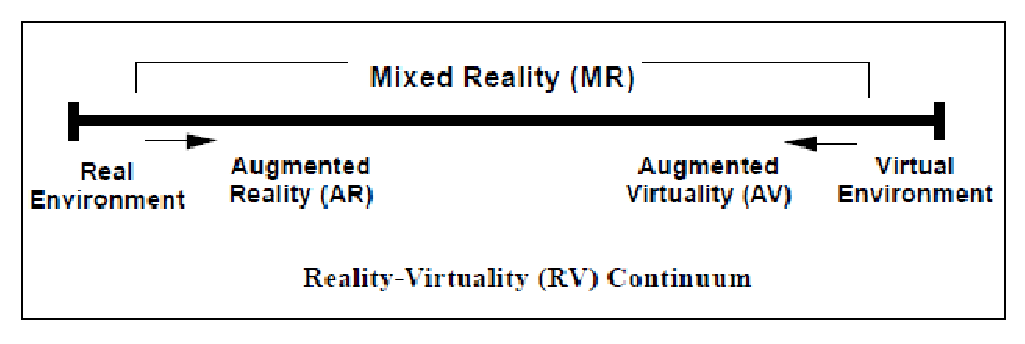
\includegraphics{../img_ent1/reality_virtual.eps}}%
\lthtmlpictureZ
\lthtmlcheckvsize\clearpage}

\stepcounter{subsection}
\stepcounter{subsubsection}
\stepcounter{subsubsection}
\stepcounter{subsection}
\stepcounter{subsection}
\stepcounter{subsection}
\stepcounter{section}
\stepcounter{subsection}
\stepcounter{subsection}
\stepcounter{section}
\stepcounter{chapter}
\stepcounter{section}
{\newpage\clearpage
\lthtmlinlinemathA{tex2html_wrap_inline12509}%
$ Z^2$%
\lthtmlinlinemathZ
\lthtmlcheckvsize\clearpage}

{\newpage\clearpage
\lthtmlinlinemathA{tex2html_wrap_inline12511}%
$ (x,y)$%
\lthtmlinlinemathZ
\lthtmlcheckvsize\clearpage}

{\newpage\clearpage
\lthtmlinlinemathA{tex2html_wrap_inline12513}%
$ A$%
\lthtmlinlinemathZ
\lthtmlcheckvsize\clearpage}

{\newpage\clearpage
\lthtmlinlinemathA{tex2html_wrap_inline12517}%
$ a=(a_1,a_2)$%
\lthtmlinlinemathZ
\lthtmlcheckvsize\clearpage}

{\newpage\clearpage
\lthtmlinlinemathA{tex2html_wrap_inline12521}%
$ \varnothing$%
\lthtmlinlinemathZ
\lthtmlcheckvsize\clearpage}

{\newpage\clearpage
\lthtmlinlinemathA{tex2html_wrap_inline12523}%
$ A \subseteq B$%
\lthtmlinlinemathZ
\lthtmlcheckvsize\clearpage}

{\newpage\clearpage
\lthtmlinlinemathA{tex2html_wrap_inline12527}%
$ B$%
\lthtmlinlinemathZ
\lthtmlcheckvsize\clearpage}

{\newpage\clearpage
\lthtmlinlinemathA{tex2html_wrap_inline12529}%
$ A \cap B$%
\lthtmlinlinemathZ
\lthtmlcheckvsize\clearpage}

{\newpage\clearpage
\lthtmlinlinemathA{tex2html_wrap_inline12539}%
$ \hat{B}=\{w|w=-b, \; \textrm{para} \; b \in B\}$%
\lthtmlinlinemathZ
\lthtmlcheckvsize\clearpage}

{\newpage\clearpage
\lthtmlinlinemathA{tex2html_wrap_inline12543}%
$ (A)_{z}=\{c|c=a+z,\; \textrm{para}\; a \in A\}$%
\lthtmlinlinemathZ
\lthtmlcheckvsize\clearpage}

{\newpage\clearpage
\lthtmlinlinemathA{tex2html_wrap_inline12547}%
$ z=(z_1, z_2)$%
\lthtmlinlinemathZ
\lthtmlcheckvsize\clearpage}

{\newpage\clearpage
\lthtmlinlinemathA{tex2html_wrap_inline12549}%
$ \{\cdot\}$%
\lthtmlinlinemathZ
\lthtmlcheckvsize\clearpage}

\stepcounter{subsection}
{\newpage\clearpage
\lthtmlinlinemathA{tex2html_wrap_inline12562}%
$ A \oplus B$%
\lthtmlinlinemathZ
\lthtmlcheckvsize\clearpage}

{\newpage\clearpage
\lthtmlinlinemathA{tex2html_wrap_indisplay12564}%
$\displaystyle A\oplus B=\{z|(\hat{B})_{z}\cap\; A \neq \varnothing\},$%
\lthtmlindisplaymathZ
\lthtmlcheckvsize\clearpage}

\stepcounter{subsection}
{\newpage\clearpage
\lthtmlinlinemathA{tex2html_wrap_inline12579}%
$ A \ominus B$%
\lthtmlinlinemathZ
\lthtmlcheckvsize\clearpage}

{\newpage\clearpage
\lthtmlinlinemathA{tex2html_wrap_indisplay12581}%
$\displaystyle A \ominus B=\{z|(B)_{z} \subseteq A\}.$%
\lthtmlindisplaymathZ
\lthtmlcheckvsize\clearpage}

{\newpage\clearpage
\lthtmlinlinemathA{tex2html_wrap_inline12587}%
$ z$%
\lthtmlinlinemathZ
\lthtmlcheckvsize\clearpage}

{\newpage\clearpage
\lthtmlpictureA{tex2html_wrap12594}%

\includegraphics[width=2.3in]{../figs/erode_dilate/orig}%
\lthtmlpictureZ
\lthtmlcheckvsize\clearpage}

{\newpage\clearpage
\lthtmlinlinemathA{tex2html_wrap_inline12596}%
$ 3\times3$%
\lthtmlinlinemathZ
\lthtmlcheckvsize\clearpage}

{\newpage\clearpage
\lthtmlpictureA{tex2html_wrap12597}%
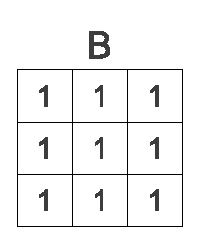
\includegraphics[width=1.0in]{../figs/mascara}%
\lthtmlpictureZ
\lthtmlcheckvsize\clearpage}

{\newpage\clearpage
\lthtmlinlinemathA{tex2html_wrap_inline12599}%
$ \times$%
\lthtmlinlinemathZ
\lthtmlcheckvsize\clearpage}

{\newpage\clearpage
\lthtmlpictureA{tex2html_wrap12600}%
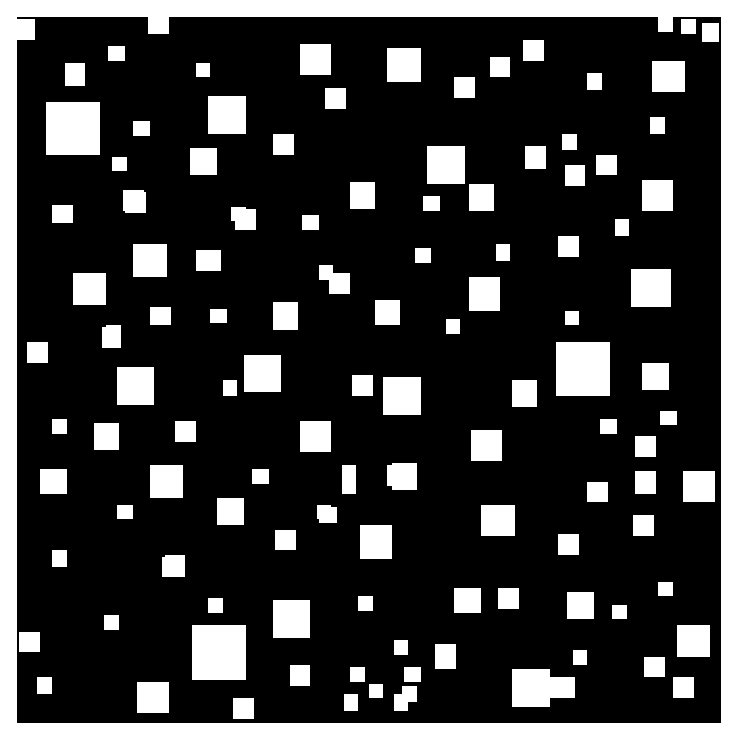
\includegraphics[width=2.3in]{../figs/erode_dilate/2dilate}%
\lthtmlpictureZ
\lthtmlcheckvsize\clearpage}

{\newpage\clearpage
\lthtmlpictureA{tex2html_wrap12603}%

\includegraphics[width=2.3in]{../figs/erode_dilate/2erode}%
\lthtmlpictureZ
\lthtmlcheckvsize\clearpage}

{\newpage\clearpage
\lthtmlinlinemathA{tex2html_wrap_inline12607}%
$ \times2$%
\lthtmlinlinemathZ
\lthtmlcheckvsize\clearpage}

\stepcounter{section}
{\newpage\clearpage
\lthtmlinlinemathA{tex2html_wrap_inline12613}%
$ g(x,y)=T[f(x,y)]$%
\lthtmlinlinemathZ
\lthtmlcheckvsize\clearpage}

{\newpage\clearpage
\lthtmlinlinemathA{tex2html_wrap_inline12615}%
$ f(x,y)$%
\lthtmlinlinemathZ
\lthtmlcheckvsize\clearpage}

{\newpage\clearpage
\lthtmlinlinemathA{tex2html_wrap_inline12617}%
$ g(x,y)$%
\lthtmlinlinemathZ
\lthtmlcheckvsize\clearpage}

{\newpage\clearpage
\lthtmlinlinemathA{tex2html_wrap_inline12619}%
$ T$%
\lthtmlinlinemathZ
\lthtmlcheckvsize\clearpage}

{\newpage\clearpage
\lthtmlinlinemathA{tex2html_wrap_inline12621}%
$ f$%
\lthtmlinlinemathZ
\lthtmlcheckvsize\clearpage}

{\newpage\clearpage
\lthtmlinlinemathA{tex2html_wrap_inline12629}%
$ 1 \times 1$%
\lthtmlinlinemathZ
\lthtmlcheckvsize\clearpage}

{\newpage\clearpage
\lthtmlinlinemathA{tex2html_wrap_inline12631}%
$ g$%
\lthtmlinlinemathZ
\lthtmlcheckvsize\clearpage}

{\newpage\clearpage
\lthtmlinlinemathA{tex2html_wrap_inline12639}%
$ s=T(r)$%
\lthtmlinlinemathZ
\lthtmlcheckvsize\clearpage}

{\newpage\clearpage
\lthtmlinlinemathA{tex2html_wrap_inline12641}%
$ r$%
\lthtmlinlinemathZ
\lthtmlcheckvsize\clearpage}

{\newpage\clearpage
\lthtmlinlinemathA{tex2html_wrap_inline12643}%
$ s$%
\lthtmlinlinemathZ
\lthtmlcheckvsize\clearpage}

\stepcounter{subsection}
{\newpage\clearpage
\lthtmlinlinemathA{tex2html_wrap_inline12652}%
$ r_{max}$%
\lthtmlinlinemathZ
\lthtmlcheckvsize\clearpage}

{\newpage\clearpage
\lthtmlinlinemathA{tex2html_wrap_inline12654}%
$ s_{max}$%
\lthtmlinlinemathZ
\lthtmlcheckvsize\clearpage}

{\newpage\clearpage
\lthtmlinlinemathA{tex2html_wrap_inline12660}%
$ u$%
\lthtmlinlinemathZ
\lthtmlcheckvsize\clearpage}

{\newpage\clearpage
\lthtmlinlinemathA{tex2html_wrap_indisplay12667}%
$\displaystyle s=  \begin{cases} 0 & \text{para $r<u$,} \\s_{max} &\text{para $r>=u$} \end{cases} \textrm{con } 0 \leq r \leq r_{max} \textrm{ y } 0 \leq u \leq r_{max}.$%
\lthtmlindisplaymathZ
\lthtmlcheckvsize\clearpage}

{\newpage\clearpage
\lthtmlpictureA{tex2html_wrap12671}%
\includegraphics[scale=1.0]{../figs/iluminacion/umbral}%
\lthtmlpictureZ
\lthtmlcheckvsize\clearpage}

\stepcounter{subsection}
{\newpage\clearpage
\lthtmlinlinemathA{tex2html_wrap_inline12678}%
$ r \geq 0$%
\lthtmlinlinemathZ
\lthtmlcheckvsize\clearpage}

{\newpage\clearpage
\lthtmlinlinemathA{tex2html_wrap_inline12680}%
$ c$%
\lthtmlinlinemathZ
\lthtmlcheckvsize\clearpage}

{\newpage\clearpage
\lthtmlinlinemathA{tex2html_wrap_inline12682}%
$ c=1$%
\lthtmlinlinemathZ
\lthtmlcheckvsize\clearpage}

{\newpage\clearpage
\lthtmlinlinemathA{tex2html_wrap_indisplay12684}%
$\displaystyle s=c\;log(1+r).$%
\lthtmlindisplaymathZ
\lthtmlcheckvsize\clearpage}

{\newpage\clearpage
\lthtmlpictureA{tex2html_wrap12688}%
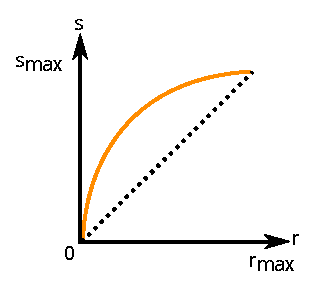
\includegraphics[scale=1.0]{../figs/iluminacion/logaritmo}%
\lthtmlpictureZ
\lthtmlcheckvsize\clearpage}

\stepcounter{subsection}
{\newpage\clearpage
\lthtmlinlinemathA{tex2html_wrap_inline12691}%
$ n$%
\lthtmlinlinemathZ
\lthtmlcheckvsize\clearpage}

{\newpage\clearpage
\lthtmlinlinemathA{tex2html_wrap_inline12693}%
$ p$%
\lthtmlinlinemathZ
\lthtmlcheckvsize\clearpage}

{\newpage\clearpage
\lthtmlinlinemathA{tex2html_wrap_inline12695}%
$ L$%
\lthtmlinlinemathZ
\lthtmlcheckvsize\clearpage}

{\newpage\clearpage
\lthtmlinlinemathA{tex2html_wrap_inline12699}%
$ k$%
\lthtmlinlinemathZ
\lthtmlcheckvsize\clearpage}

{\newpage\clearpage
\lthtmlinlinemathA{tex2html_wrap_inline12701}%
$ r_k$%
\lthtmlinlinemathZ
\lthtmlcheckvsize\clearpage}

{\newpage\clearpage
\lthtmlinlinemathA{tex2html_wrap_inline12703}%
$ r_{k}=0,\frac{1}{2^{p}-1},\frac{2}{2^{p}-1},\ldots,1.$%
\lthtmlinlinemathZ
\lthtmlcheckvsize\clearpage}

{\newpage\clearpage
\lthtmlinlinemathA{tex2html_wrap_inline12705}%
$ p_{r}(r_{k})$%
\lthtmlinlinemathZ
\lthtmlcheckvsize\clearpage}

{\newpage\clearpage
\lthtmlinlinemathA{tex2html_wrap_indisplay12707}%
$\displaystyle p_{r}(r_{k})=\frac{n_{k}}{n},\; \textrm{con}\begin{cases} \begin{array}{c} 0\leq r_{k}\leq1\\k=0,1,\ldots,L-1 \end{array},\end{cases}$%
\lthtmlindisplaymathZ
\lthtmlcheckvsize\clearpage}

{\newpage\clearpage
\lthtmlinlinemathA{tex2html_wrap_indisplay12709}%
$\displaystyle s_{k}(r_{k})=T(r_{k})=\sum_{j=0}^{k}\frac{n_{j}}{n}=\sum_{j=0}^{k}p_{r}(r_{j}),\; \textrm{con}\begin{cases} \begin{array}{c} 0\leq r_{k}\leq1\\k=0,1,\ldots,L-1 \end{array}.\end{cases}$%
\lthtmlindisplaymathZ
\lthtmlcheckvsize\clearpage}

\stepcounter{subsection}
{\newpage\clearpage
\lthtmlinlinemathA{tex2html_wrap_inline12712}%
$ f(x+s, y+t)$%
\lthtmlinlinemathZ
\lthtmlcheckvsize\clearpage}

{\newpage\clearpage
\lthtmlinlinemathA{tex2html_wrap_inline12714}%
$ w(s,t)$%
\lthtmlinlinemathZ
\lthtmlcheckvsize\clearpage}

{\newpage\clearpage
\lthtmlinlinemathA{tex2html_wrap_indisplay12716}%
$\displaystyle g(x,y)=\sum_{s=-a}^{a}\sum_{\; t=-b}^{a}w(s,t)f(x+s,y+t).$%
\lthtmlindisplaymathZ
\lthtmlcheckvsize\clearpage}

\stepcounter{subsection}
{\newpage\clearpage
\lthtmlinlinemathA{tex2html_wrap_inline12719}%
$ A \geq 1$%
\lthtmlinlinemathZ
\lthtmlcheckvsize\clearpage}

{\newpage\clearpage
\lthtmlinlinemathA{tex2html_wrap_inline12723}%
$ PB(f(x,y))$%
\lthtmlinlinemathZ
\lthtmlcheckvsize\clearpage}

{\newpage\clearpage
\lthtmlinlinemathA{tex2html_wrap_inline12729}%
$ A=1$%
\lthtmlinlinemathZ
\lthtmlcheckvsize\clearpage}

{\newpage\clearpage
\lthtmldisplayA{displaymath12732}%
\begin{equation*}\begin{aligned}
g(x,y)&=Af(x,y)-PB(f(x,y))\\
&= (A-1)f(x,y)+PA(f(x,y)).
\end{aligned}\end{equation*}%
\lthtmldisplayZ
\lthtmlcheckvsize\clearpage}

\stepcounter{section}
\stepcounter{subsubsection}
{\newpage\clearpage
\lthtmlinlinemathA{tex2html_wrap_inline12736}%
$ \mathit{I_{\sum}(\mathbf{x})}$%
\lthtmlinlinemathZ
\lthtmlcheckvsize\clearpage}

{\newpage\clearpage
\lthtmlinlinemathA{tex2html_wrap_inline12738}%
$ \mathbf{x}=(x,y)^{T}$%
\lthtmlinlinemathZ
\lthtmlcheckvsize\clearpage}

{\newpage\clearpage
\lthtmlinlinemathA{tex2html_wrap_inline12740}%
$ \mathit{I}$%
\lthtmlinlinemathZ
\lthtmlcheckvsize\clearpage}

{\newpage\clearpage
\lthtmlinlinemathA{tex2html_wrap_inline12742}%
$ \mathbf{x}$%
\lthtmlinlinemathZ
\lthtmlcheckvsize\clearpage}

{\newpage\clearpage
\lthtmlinlinemathA{tex2html_wrap_indisplay12744}%
$\displaystyle \mathit{I}_{\sum}(\mathbf{x})=\sum_{i=0}^{i\leq x}\quad\sum_{j=0}^{j\leq y}I(i,j).$%
\lthtmlindisplaymathZ
\lthtmlcheckvsize\clearpage}

{\newpage\clearpage
\lthtmlpictureA{tex2html_wrap12748}%
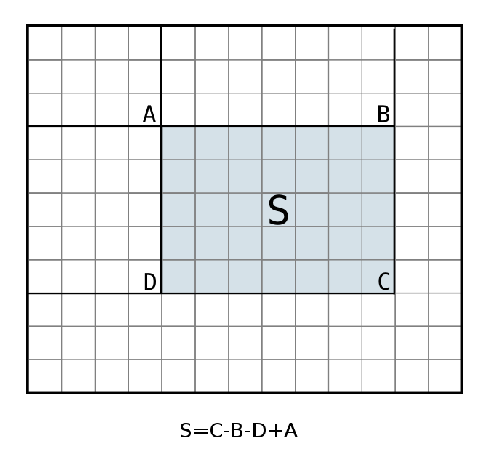
\includegraphics[scale=0.6]{./figs/sumintegralimages2}%
\lthtmlpictureZ
\lthtmlcheckvsize\clearpage}

\stepcounter{subsection}
\stepcounter{subsubsection}
{\newpage\clearpage
\lthtmlinlinemathA{tex2html_wrap_inline12753}%
$ \sigma$%
\lthtmlinlinemathZ
\lthtmlcheckvsize\clearpage}

{\newpage\clearpage
\lthtmlpictureA{tex2html_wrap12758}%
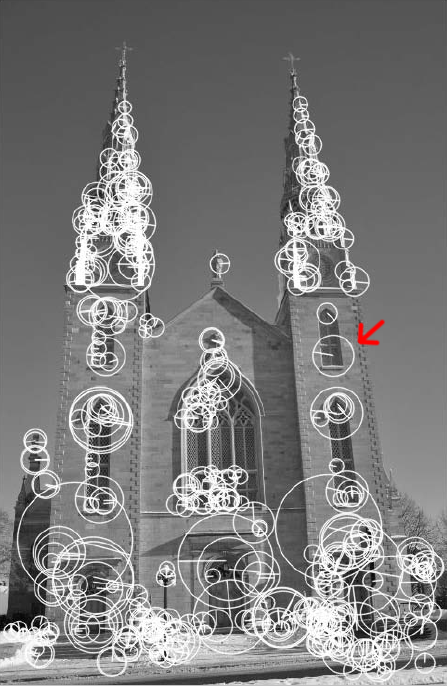
\includegraphics[scale=0.338]{../img_ent2/surfinchurch1}%
\lthtmlpictureZ
\lthtmlcheckvsize\clearpage}

{\newpage\clearpage
\lthtmlpictureA{tex2html_wrap12759}%
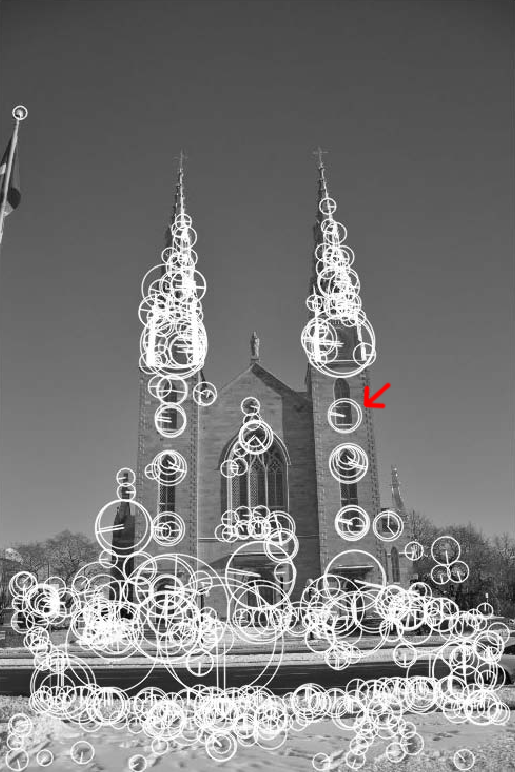
\includegraphics[scale=0.3]{../img_ent2/surfinchurch2}%
\lthtmlpictureZ
\lthtmlcheckvsize\clearpage}

\stepcounter{subsection}
{\newpage\clearpage
\lthtmlinlinemathA{tex2html_wrap_indisplay12765}%
$\displaystyle H(x,y)=\begin{bmatrix}\frac{\partial^{2}I}{\partial x\text{\texttwosuperior}} & \frac{\partial^{2}I}{\partial x\partial y}\\& \\\frac{\partial^{2}I}{\partial y\partial x} & \frac{\partial^{2}I}{\partial y\text{\texttwosuperior}} 	\end{bmatrix};\; \textrm{con}\; \frac{\partial^{2}I}{\partial x\partial y}=\frac{\partial^{2}I}{\partial y\partial x}.$%
\lthtmlindisplaymathZ
\lthtmlcheckvsize\clearpage}

{\newpage\clearpage
\lthtmlinlinemathA{tex2html_wrap_inline12767}%
$ \mathbf{p}=(x,y)$%
\lthtmlinlinemathZ
\lthtmlcheckvsize\clearpage}

{\newpage\clearpage
\lthtmlinlinemathA{tex2html_wrap_inline12771}%
$ \mathbf{p}$%
\lthtmlinlinemathZ
\lthtmlcheckvsize\clearpage}

{\newpage\clearpage
\lthtmlinlinemathA{tex2html_wrap_indisplay12775}%
$\displaystyle \mathcal{H}(\mathbf{p},\sigma)=\left[\begin{array}{cc}       \mathit{L_{xx}(\mathbf{p},}\sigma)\hphantom{} & \mathit{L_{xy}(\mathbf{p},}\sigma)\\\mathit{L_{xy}(\mathbf{p},}\sigma)\hphantom{} & \mathit{L_{yy}(\mathbf{p},}\sigma)       \end{array}\right],$%
\lthtmlindisplaymathZ
\lthtmlcheckvsize\clearpage}

{\newpage\clearpage
\lthtmlinlinemathA{tex2html_wrap_inline12777}%
$ \mathit{L_{xx}(\mathbf{p},}\sigma)$%
\lthtmlinlinemathZ
\lthtmlcheckvsize\clearpage}

{\newpage\clearpage
\lthtmlinlinemathA{tex2html_wrap_inline12779}%
$ \frac{\partial^{2}}{\partial x^{2}}\mathit{g}(\sigma)$%
\lthtmlinlinemathZ
\lthtmlcheckvsize\clearpage}

{\newpage\clearpage
\lthtmlinlinemathA{tex2html_wrap_inline12785}%
$ \mathit{L_{xy}(\mathbf{p},}\sigma)$%
\lthtmlinlinemathZ
\lthtmlcheckvsize\clearpage}

{\newpage\clearpage
\lthtmlinlinemathA{tex2html_wrap_inline12787}%
$ \frac{\partial^{2}}{\partial x \partial y}\mathit{g}(\sigma)$%
\lthtmlinlinemathZ
\lthtmlcheckvsize\clearpage}

{\newpage\clearpage
\lthtmlinlinemathA{tex2html_wrap_inline12793}%
$ \mathit{L_{yy}(\mathbf{p},}\sigma)$%
\lthtmlinlinemathZ
\lthtmlcheckvsize\clearpage}

{\newpage\clearpage
\lthtmlinlinemathA{tex2html_wrap_inline12795}%
$ \frac{\partial^{2}}{\partial y^{2}}\mathit{g}(\sigma)$%
\lthtmlinlinemathZ
\lthtmlcheckvsize\clearpage}

{\newpage\clearpage
\lthtmlpictureA{tex2html_wrap12803}%
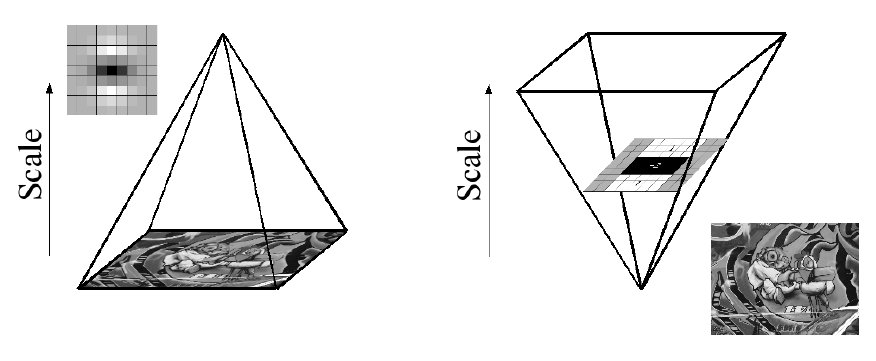
\includegraphics[scale=0.6]{./figs/pyramidfilters}%
\lthtmlpictureZ
\lthtmlcheckvsize\clearpage}

{\newpage\clearpage
\lthtmlinlinemathA{tex2html_wrap_indisplay12805}%
$\displaystyle \det(\mathcal{H}_{approximado})=D_{xx}D_{yy}-(wD_{xy})^{2}$%
\lthtmlindisplaymathZ
\lthtmlcheckvsize\clearpage}

{\newpage\clearpage
\lthtmlinlinemathA{tex2html_wrap_inline12807}%
$ w=0.9$%
\lthtmlinlinemathZ
\lthtmlcheckvsize\clearpage}

{\newpage\clearpage
\lthtmlinlinemathA{tex2html_wrap_inline12809}%
$ \mathit{D}_{xx}$%
\lthtmlinlinemathZ
\lthtmlcheckvsize\clearpage}

{\newpage\clearpage
\lthtmlinlinemathA{tex2html_wrap_inline12811}%
$ \mathit{D}_{yy}$%
\lthtmlinlinemathZ
\lthtmlcheckvsize\clearpage}

{\newpage\clearpage
\lthtmlinlinemathA{tex2html_wrap_inline12813}%
$ \mathit{D}_{xy}$%
\lthtmlinlinemathZ
\lthtmlcheckvsize\clearpage}

{\newpage\clearpage
\lthtmlinlinemathA{tex2html_wrap_inline12815}%
$ w$%
\lthtmlinlinemathZ
\lthtmlcheckvsize\clearpage}

{\newpage\clearpage
\lthtmlinlinemathA{tex2html_wrap_inline12819}%
$ L_{yy}$%
\lthtmlinlinemathZ
\lthtmlcheckvsize\clearpage}

{\newpage\clearpage
\lthtmlinlinemathA{tex2html_wrap_inline12821}%
$ D_{yy}$%
\lthtmlinlinemathZ
\lthtmlcheckvsize\clearpage}

{\newpage\clearpage
\lthtmlinlinemathA{tex2html_wrap_inline12823}%
$ L_{xy}$%
\lthtmlinlinemathZ
\lthtmlcheckvsize\clearpage}

{\newpage\clearpage
\lthtmlinlinemathA{tex2html_wrap_inline12825}%
$ D_{xy}$%
\lthtmlinlinemathZ
\lthtmlcheckvsize\clearpage}

{\newpage\clearpage
\lthtmlpictureA{tex2html_wrap12826}%
\includegraphics[scale=0.45]{../img_ent2/gaussiankernelsdiscrete_y}%
\lthtmlpictureZ
\lthtmlcheckvsize\clearpage}

{\newpage\clearpage
\lthtmlpictureA{tex2html_wrap12827}%
\includegraphics[scale=0.45]{../img_ent2/gaussiankernelsaprox_y}%
\lthtmlpictureZ
\lthtmlcheckvsize\clearpage}

{\newpage\clearpage
\lthtmlpictureA{tex2html_wrap12828}%
\includegraphics[scale=0.45]{../img_ent2/gaussiankernelsdiscrete_xy}%
\lthtmlpictureZ
\lthtmlcheckvsize\clearpage}

{\newpage\clearpage
\lthtmlpictureA{tex2html_wrap12829}%
\includegraphics[scale=0.45]{../img_ent2/gaussiankernelsaprox_xy}%
\lthtmlpictureZ
\lthtmlcheckvsize\clearpage}

{\newpage\clearpage
\lthtmlinlinemathA{tex2html_wrap_inline12834}%
$ 9 \times 9$%
\lthtmlinlinemathZ
\lthtmlcheckvsize\clearpage}

{\newpage\clearpage
\lthtmlinlinemathA{tex2html_wrap_inline12836}%
$ \sigma=1.2$%
\lthtmlinlinemathZ
\lthtmlcheckvsize\clearpage}

{\newpage\clearpage
\lthtmlinlinemathA{tex2html_wrap_inline12838}%
$ s=1.2$%
\lthtmlinlinemathZ
\lthtmlcheckvsize\clearpage}

{\newpage\clearpage
\lthtmlinlinemathA{tex2html_wrap_inline12842}%
$ 15 \times 15$%
\lthtmlinlinemathZ
\lthtmlcheckvsize\clearpage}

{\newpage\clearpage
\lthtmlinlinemathA{tex2html_wrap_inline12844}%
$ 21 \times 21$%
\lthtmlinlinemathZ
\lthtmlcheckvsize\clearpage}

{\newpage\clearpage
\lthtmlinlinemathA{tex2html_wrap_inline12846}%
$ 27 \times 27$%
\lthtmlinlinemathZ
\lthtmlcheckvsize\clearpage}

{\newpage\clearpage
\lthtmlinlinemathA{tex2html_wrap_inline12850}%
$ \sigma = 1.6$%
\lthtmlinlinemathZ
\lthtmlcheckvsize\clearpage}

{\newpage\clearpage
\lthtmlinlinemathA{tex2html_wrap_inline12852}%
$ 12 \times 12$%
\lthtmlinlinemathZ
\lthtmlcheckvsize\clearpage}

{\newpage\clearpage
\lthtmlinlinemathA{tex2html_wrap_inline12854}%
$ \sigma = 3.2$%
\lthtmlinlinemathZ
\lthtmlcheckvsize\clearpage}

{\newpage\clearpage
\lthtmlinlinemathA{tex2html_wrap_inline12856}%
$ 24 \times 24$%
\lthtmlinlinemathZ
\lthtmlcheckvsize\clearpage}

{\newpage\clearpage
\lthtmlpictureA{tex2html_wrap12860}%
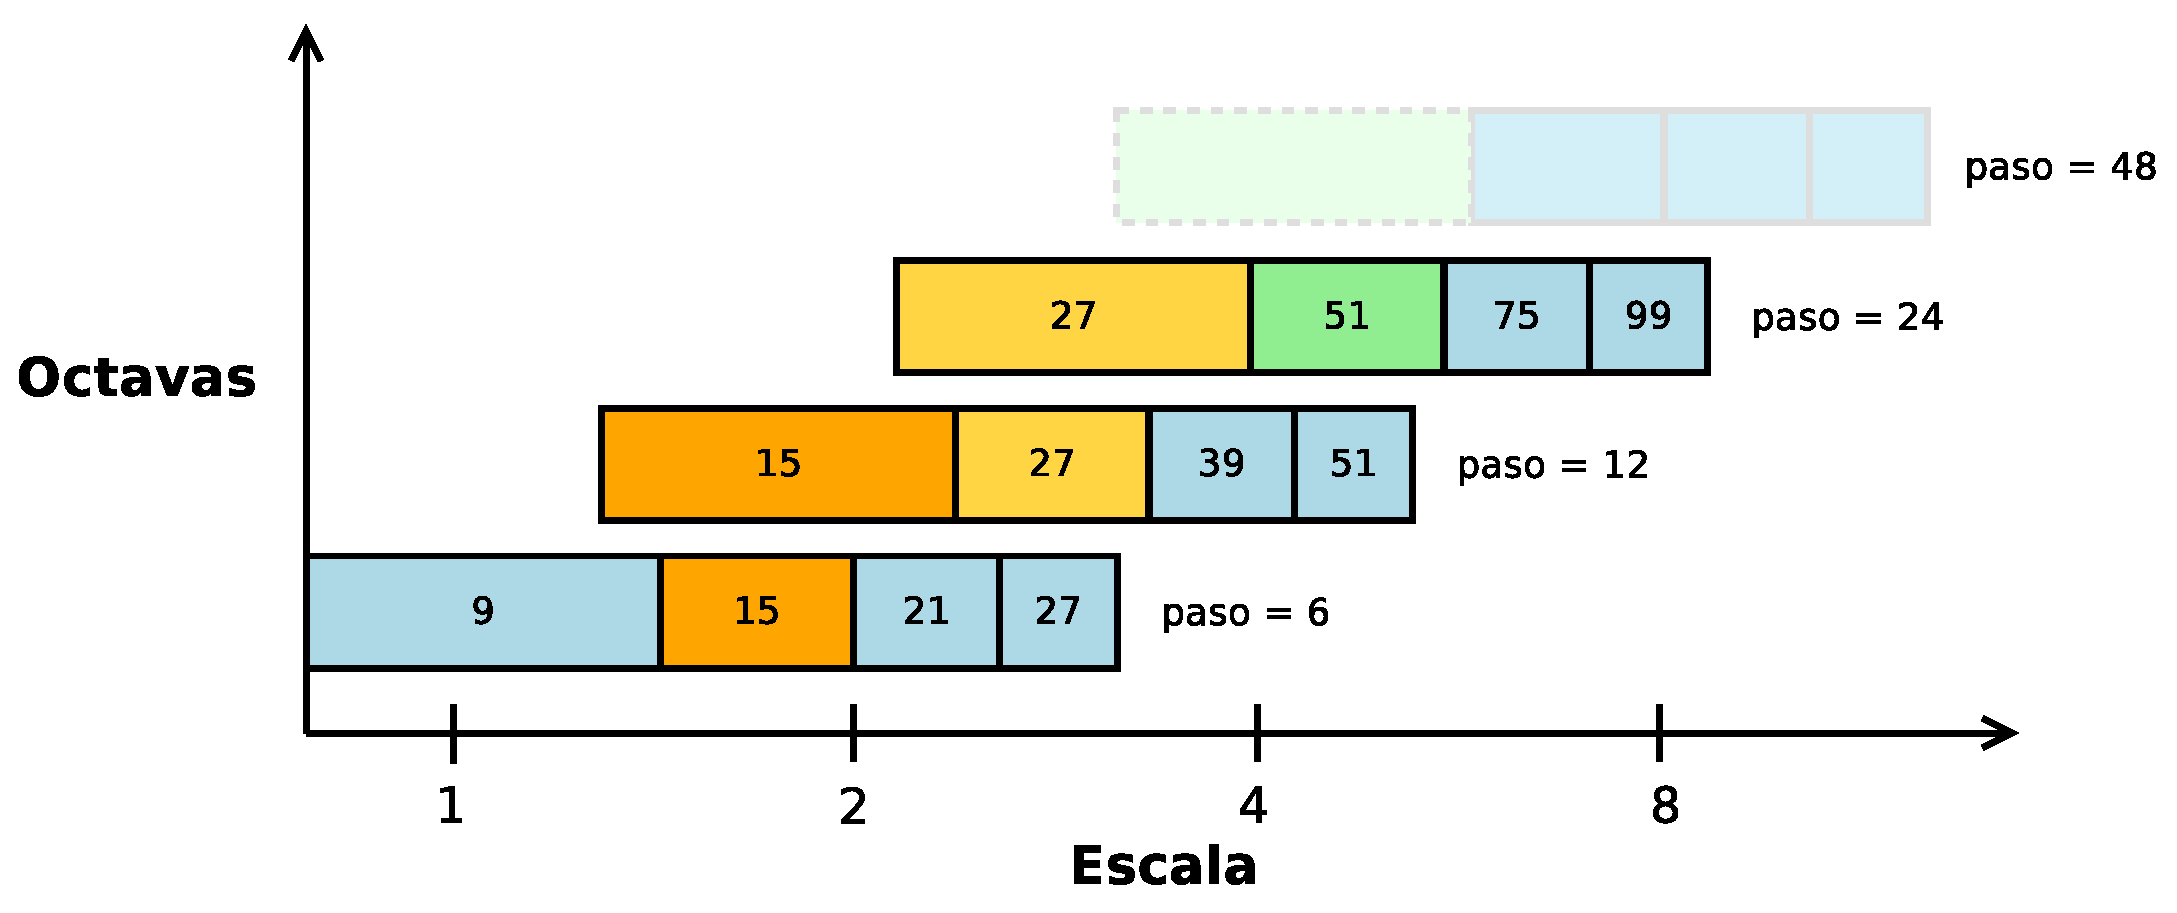
\includegraphics[scale=0.32]{./figs/tamfilters1}%
\lthtmlpictureZ
\lthtmlcheckvsize\clearpage}

\stepcounter{subsection}
{\newpage\clearpage
\lthtmlinlinemathA{tex2html_wrap_inline12863}%
$ 2 \times 9$%
\lthtmlinlinemathZ
\lthtmlcheckvsize\clearpage}

{\newpage\clearpage
\lthtmlinlinemathA{tex2html_wrap_inline12865}%
$ 3 \times 3 \times 3$%
\lthtmlinlinemathZ
\lthtmlcheckvsize\clearpage}

{\newpage\clearpage
\lthtmlinlinemathA{tex2html_wrap_inline12869}%
$ \sigma=k$%
\lthtmlinlinemathZ
\lthtmlcheckvsize\clearpage}

{\newpage\clearpage
\lthtmlinlinemathA{tex2html_wrap_inline12871}%
$ \sigma=\frac{3}{2}k$%
\lthtmlinlinemathZ
\lthtmlcheckvsize\clearpage}

{\newpage\clearpage
\lthtmlinlinemathA{tex2html_wrap_inline12873}%
$ \sigma=2k$%
\lthtmlinlinemathZ
\lthtmlcheckvsize\clearpage}

{\newpage\clearpage
\lthtmlpictureA{tex2html_wrap12875}%
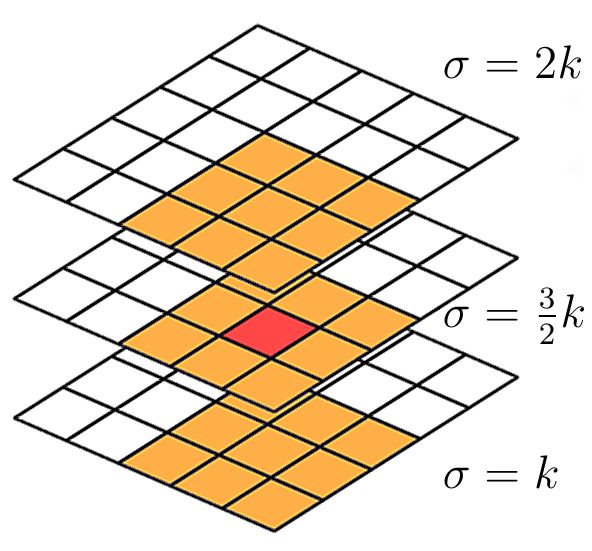
\includegraphics[scale=0.35]{./figs/333nonmaximum}%
\lthtmlpictureZ
\lthtmlcheckvsize\clearpage}

\stepcounter{section}
\stepcounter{subsection}
{\newpage\clearpage
\lthtmlinlinemathA{tex2html_wrap_inline12879}%
$ 6s$%
\lthtmlinlinemathZ
\lthtmlcheckvsize\clearpage}

{\newpage\clearpage
\lthtmlinlinemathA{tex2html_wrap_inline12885}%
$ 4s$%
\lthtmlinlinemathZ
\lthtmlcheckvsize\clearpage}

{\newpage\clearpage
\lthtmlinlinemathA{tex2html_wrap_inline12887}%
$ \sigma=2s$%
\lthtmlinlinemathZ
\lthtmlcheckvsize\clearpage}

{\newpage\clearpage
\lthtmlpictureA{tex2html_wrap12888}%
\includegraphics[scale=0.4]{../img_ent2/simplekernels1harn}%
\lthtmlpictureZ
\lthtmlcheckvsize\clearpage}

{\newpage\clearpage
\lthtmlpictureA{tex2html_wrap12889}%
\includegraphics[scale=0.4]{../img_ent2/simplekernels2harn}%
\lthtmlpictureZ
\lthtmlcheckvsize\clearpage}

{\newpage\clearpage
\lthtmlinlinemathA{tex2html_wrap_inline12893}%
$ x$%
\lthtmlinlinemathZ
\lthtmlcheckvsize\clearpage}

{\newpage\clearpage
\lthtmlinlinemathA{tex2html_wrap_inline12895}%
$ y$%
\lthtmlinlinemathZ
\lthtmlcheckvsize\clearpage}

{\newpage\clearpage
\lthtmlinlinemathA{tex2html_wrap_inline12898}%
$ dx$%
\lthtmlinlinemathZ
\lthtmlcheckvsize\clearpage}

{\newpage\clearpage
\lthtmlinlinemathA{tex2html_wrap_inline12900}%
$ dy$%
\lthtmlinlinemathZ
\lthtmlcheckvsize\clearpage}

{\newpage\clearpage
\lthtmlinlinemathA{tex2html_wrap_inline12902}%
$ \pi/3$%
\lthtmlinlinemathZ
\lthtmlcheckvsize\clearpage}

{\newpage\clearpage
\lthtmlinlinemathA{tex2html_wrap_inline12906}%
$ \frac{\pi}{3}$%
\lthtmlinlinemathZ
\lthtmlcheckvsize\clearpage}

{\newpage\clearpage
\lthtmlpictureA{tex2html_wrap12908}%
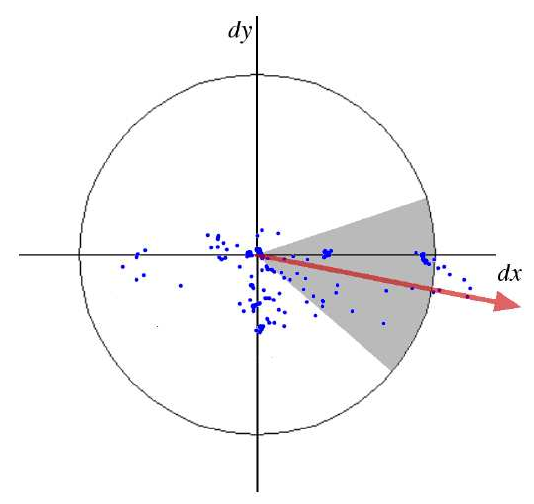
\includegraphics[scale=0.45]{./figs/responsecalculate}%
\lthtmlpictureZ
\lthtmlcheckvsize\clearpage}

\stepcounter{subsection}
{\newpage\clearpage
\lthtmlinlinemathA{tex2html_wrap_inline12911}%
$ 20s$%
\lthtmlinlinemathZ
\lthtmlcheckvsize\clearpage}

{\newpage\clearpage
\lthtmlpictureA{tex2html_wrap12915}%
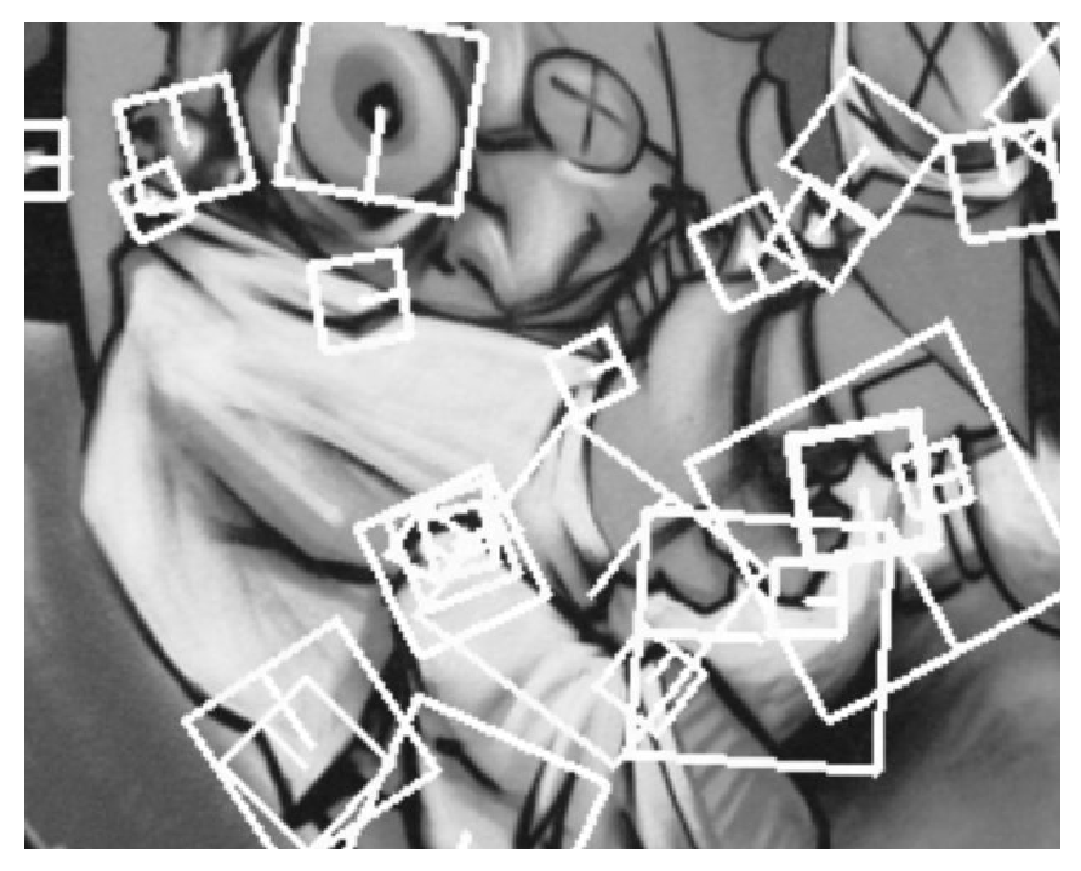
\includegraphics[scale=0.4]{./figs/squareregionsexample}%
\lthtmlpictureZ
\lthtmlcheckvsize\clearpage}

{\newpage\clearpage
\lthtmlpictureA{tex2html_wrap12916}%
\includegraphics[scale=0.30]{./figs/subdivideregions}%
\lthtmlpictureZ
\lthtmlcheckvsize\clearpage}

{\newpage\clearpage
\lthtmlpictureA{tex2html_wrap12917}%
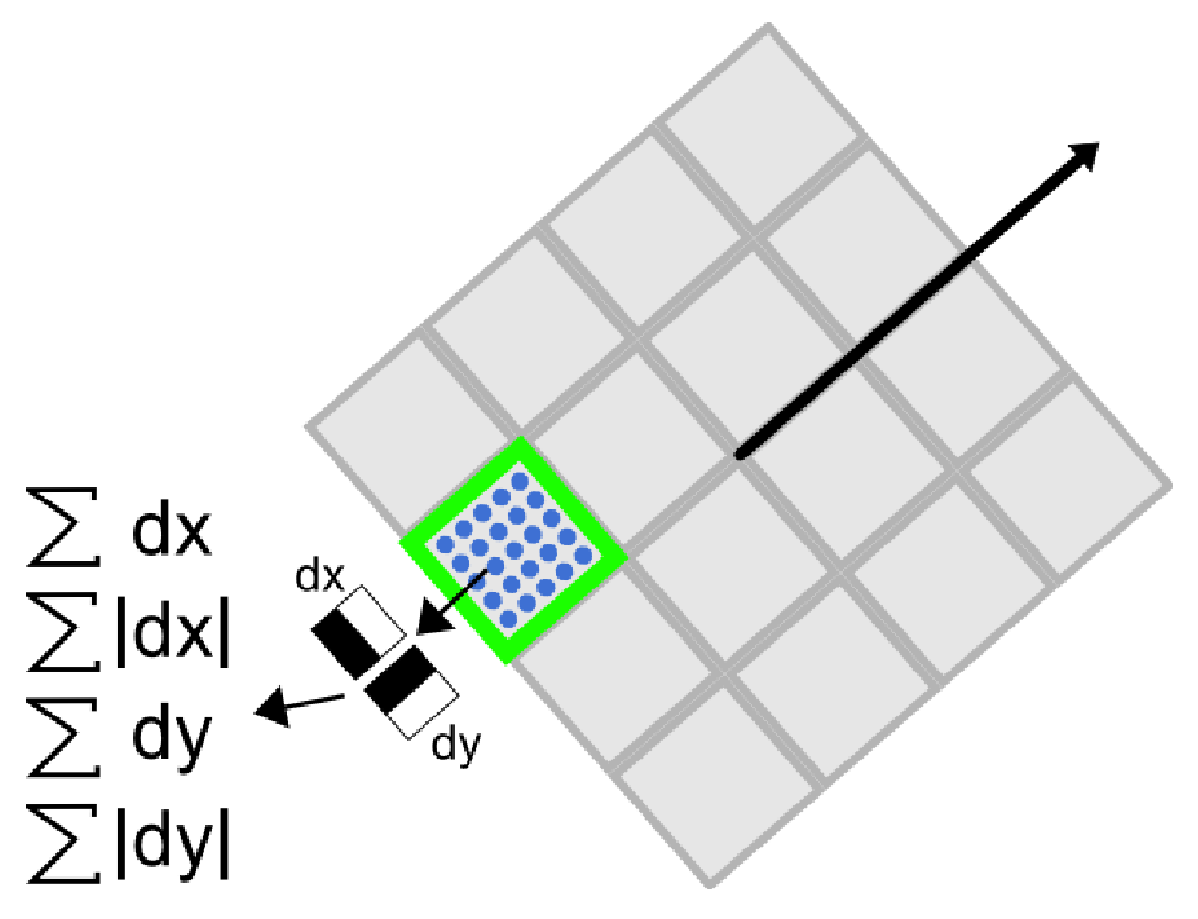
\includegraphics[scale=0.30]{./figs/respuestaswavelethaar}%
\lthtmlpictureZ
\lthtmlcheckvsize\clearpage}

{\newpage\clearpage
\lthtmlpictureA{tex2html_wrap12924}%
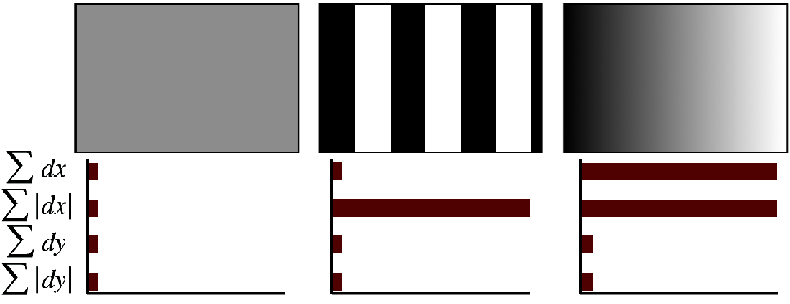
\includegraphics[scale=0.60]{./figs/descriptorresponses}%
\lthtmlpictureZ
\lthtmlcheckvsize\clearpage}

{\newpage\clearpage
\lthtmlinlinemathA{tex2html_wrap_inline12926}%
$ 4 \times 4$%
\lthtmlinlinemathZ
\lthtmlcheckvsize\clearpage}

{\newpage\clearpage
\lthtmlinlinemathA{tex2html_wrap_inline12928}%
$ 5 \times 5$%
\lthtmlinlinemathZ
\lthtmlcheckvsize\clearpage}

{\newpage\clearpage
\lthtmlinlinemathA{tex2html_wrap_inline12930}%
$ 2 \times 2$%
\lthtmlinlinemathZ
\lthtmlcheckvsize\clearpage}

{\newpage\clearpage
\lthtmlinlinemathA{tex2html_wrap_inline12934}%
$ |dx|$%
\lthtmlinlinemathZ
\lthtmlcheckvsize\clearpage}

{\newpage\clearpage
\lthtmlinlinemathA{tex2html_wrap_inline12938}%
$ |dy|$%
\lthtmlinlinemathZ
\lthtmlcheckvsize\clearpage}

{\newpage\clearpage
\lthtmlinlinemathA{tex2html_wrap_inline12940}%
$ d_x$%
\lthtmlinlinemathZ
\lthtmlcheckvsize\clearpage}

{\newpage\clearpage
\lthtmlinlinemathA{tex2html_wrap_inline12942}%
$ d_y$%
\lthtmlinlinemathZ
\lthtmlcheckvsize\clearpage}

{\newpage\clearpage
\lthtmlinlinemathA{tex2html_wrap_inline12944}%
$ 2s$%
\lthtmlinlinemathZ
\lthtmlcheckvsize\clearpage}

{\newpage\clearpage
\lthtmlinlinemathA{tex2html_wrap_inline12950}%
$ \sigma=3.3s$%
\lthtmlinlinemathZ
\lthtmlcheckvsize\clearpage}

{\newpage\clearpage
\lthtmlinlinemathA{tex2html_wrap_inline12960}%
$ \mathbf{v}$%
\lthtmlinlinemathZ
\lthtmlcheckvsize\clearpage}

{\newpage\clearpage
\lthtmlinlinemathA{tex2html_wrap_inline12962}%
$ \mathbf{v}=(\sum{d_x},\sum{d_y},\sum{|d_x|},\sum{|d_y|})$%
\lthtmlinlinemathZ
\lthtmlcheckvsize\clearpage}

{\newpage\clearpage
\lthtmlinlinemathA{tex2html_wrap_inline12964}%
$ 16$%
\lthtmlinlinemathZ
\lthtmlcheckvsize\clearpage}

{\newpage\clearpage
\lthtmlinlinemathA{tex2html_wrap_inline12968}%
$ 16 \times 4$%
\lthtmlinlinemathZ
\lthtmlcheckvsize\clearpage}

{\newpage\clearpage
\lthtmlinlinemathA{tex2html_wrap_inline12972}%
$ \sum{|d_x|}$%
\lthtmlinlinemathZ
\lthtmlcheckvsize\clearpage}

{\newpage\clearpage
\lthtmlinlinemathA{tex2html_wrap_inline12976}%
$ \sum{d_x}$%
\lthtmlinlinemathZ
\lthtmlcheckvsize\clearpage}

\stepcounter{section}
{\newpage\clearpage
\lthtmlinlinemathA{tex2html_wrap_inline12981}%
$ P=\left\{ p_{1,...,}p_{n}\right\}$%
\lthtmlinlinemathZ
\lthtmlcheckvsize\clearpage}

{\newpage\clearpage
\lthtmlinlinemathA{tex2html_wrap_inline12983}%
$ M$%
\lthtmlinlinemathZ
\lthtmlcheckvsize\clearpage}

{\newpage\clearpage
\lthtmlinlinemathA{tex2html_wrap_inline12985}%
$ q \in M$%
\lthtmlinlinemathZ
\lthtmlcheckvsize\clearpage}

{\newpage\clearpage
\lthtmlinlinemathA{tex2html_wrap_inline12987}%
$ q$%
\lthtmlinlinemathZ
\lthtmlcheckvsize\clearpage}

{\newpage\clearpage
\lthtmlinlinemathA{tex2html_wrap_inline12989}%
$ P$%
\lthtmlinlinemathZ
\lthtmlcheckvsize\clearpage}

{\newpage\clearpage
\lthtmlinlinemathA{tex2html_wrap_inline12993}%
$ K$%
\lthtmlinlinemathZ
\lthtmlcheckvsize\clearpage}

{\newpage\clearpage
\lthtmlinlinemathA{tex2html_wrap_inline12995}%
$ K=1$%
\lthtmlinlinemathZ
\lthtmlcheckvsize\clearpage}

\stepcounter{subsection}
{\newpage\clearpage
\lthtmlinlinemathA{tex2html_wrap_inline12998}%
$ D$%
\lthtmlinlinemathZ
\lthtmlcheckvsize\clearpage}

{\newpage\clearpage
\lthtmlinlinemathA{tex2html_wrap_inline13000}%
$ D=5$%
\lthtmlinlinemathZ
\lthtmlcheckvsize\clearpage}

\stepcounter{subsection}
{\newpage\clearpage
\lthtmlinlinemathA{tex2html_wrap_inline13007}%
$ a_i$%
\lthtmlinlinemathZ
\lthtmlcheckvsize\clearpage}

{\newpage\clearpage
\lthtmlinlinemathA{tex2html_wrap_inline13009}%
$ i=0\ldots n$%
\lthtmlinlinemathZ
\lthtmlcheckvsize\clearpage}

{\newpage\clearpage
\lthtmlinlinemathA{tex2html_wrap_inline13017}%
$ av_i$%
\lthtmlinlinemathZ
\lthtmlcheckvsize\clearpage}

{\newpage\clearpage
\lthtmlinlinemathA{tex2html_wrap_inline13025}%
$ p_1 \in b_i$%
\lthtmlinlinemathZ
\lthtmlcheckvsize\clearpage}

{\newpage\clearpage
\lthtmlinlinemathA{tex2html_wrap_inline13027}%
$ p_2 \in b_i$%
\lthtmlinlinemathZ
\lthtmlcheckvsize\clearpage}

{\newpage\clearpage
\lthtmlinlinemathA{tex2html_wrap_inline13029}%
$ d_1$%
\lthtmlinlinemathZ
\lthtmlcheckvsize\clearpage}

{\newpage\clearpage
\lthtmlinlinemathA{tex2html_wrap_inline13031}%
$ d_2$%
\lthtmlinlinemathZ
\lthtmlcheckvsize\clearpage}

{\newpage\clearpage
\lthtmlinlinemathA{tex2html_wrap_inline13035}%
$ \frac{d_{1}}{d_{2}}>\varepsilon\qquad(\varepsilon=0.8\:\cite{Lowe:2004:DIF:993451.996342})$%
\lthtmlinlinemathZ
\lthtmlcheckvsize\clearpage}

{\newpage\clearpage
\lthtmlinlinemathA{tex2html_wrap_inline13037}%
$ \varepsilon=0.8$%
\lthtmlinlinemathZ
\lthtmlcheckvsize\clearpage}

\stepcounter{section}
\stepcounter{subsection}
\stepcounter{subsection}
{\newpage\clearpage
\lthtmlinlinemathA{tex2html_wrap_inline13043}%
$ \mathbf{C}$%
\lthtmlinlinemathZ
\lthtmlcheckvsize\clearpage}

{\newpage\clearpage
\lthtmlinlinemathA{tex2html_wrap_inline13045}%
$ \mathsf{Z}=f$%
\lthtmlinlinemathZ
\lthtmlcheckvsize\clearpage}

{\newpage\clearpage
\lthtmlinlinemathA{tex2html_wrap_inline13049}%
$ \mathbf{X}=(\mathsf{X},\mathsf{Y},\mathsf{Z})^\mathsf{T}$%
\lthtmlinlinemathZ
\lthtmlcheckvsize\clearpage}

{\newpage\clearpage
\lthtmlinlinemathA{tex2html_wrap_inline13051}%
$ \mathbf{X}$%
\lthtmlinlinemathZ
\lthtmlcheckvsize\clearpage}

{\newpage\clearpage
\lthtmlinlinemathA{tex2html_wrap_inline13053}%
$ C$%
\lthtmlinlinemathZ
\lthtmlcheckvsize\clearpage}

{\newpage\clearpage
\lthtmlinlinemathA{tex2html_wrap_inline13057}%
$ \mathbf{x}=(\mathit{f}\mathsf{X}/\mathsf{Z}, \mathit{f}\mathsf{Y}/\mathsf{Z}, f)^\mathsf{T}$%
\lthtmlinlinemathZ
\lthtmlcheckvsize\clearpage}

{\newpage\clearpage
\lthtmlinlinemathA{tex2html_wrap_inline13059}%
$ \mathbb{R}^3$%
\lthtmlinlinemathZ
\lthtmlcheckvsize\clearpage}

{\newpage\clearpage
\lthtmlinlinemathA{tex2html_wrap_inline13061}%
$ \mathbb{R}^2$%
\lthtmlinlinemathZ
\lthtmlcheckvsize\clearpage}

{\newpage\clearpage
\lthtmlinlinemathA{tex2html_wrap_indisplay13063}%
$\displaystyle (\mathsf{X},\mathsf{Y},\mathsf{Z}) \mapsto (\mathit{f}\mathsf{X}/\mathsf{Z}, \mathit{f}\mathsf{Y}/\mathsf{Z})^\mathsf{T}.$%
\lthtmlindisplaymathZ
\lthtmlcheckvsize\clearpage}

{\newpage\clearpage
\lthtmlpictureA{tex2html_wrap13064}%
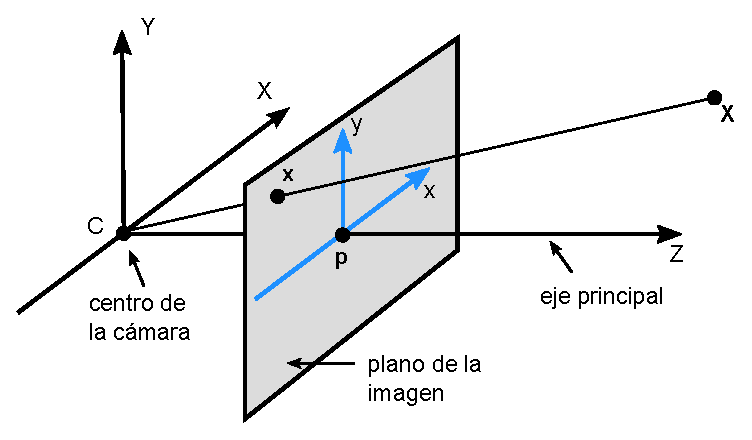
\includegraphics[scale=0.6]{../figs/sizzerman/pinholemodel}%
\lthtmlpictureZ
\lthtmlcheckvsize\clearpage}

{\newpage\clearpage
\lthtmlpictureA{tex2html_wrap13065}%
\includegraphics[scale=0.6]{../figs/sizzerman/pinholemodelgeometria}%
\lthtmlpictureZ
\lthtmlcheckvsize\clearpage}

{\newpage\clearpage
\lthtmlinlinemathA{tex2html_wrap_indisplay13070}%
$\displaystyle \left(\begin{array}{c} \mathsf{X}\\\mathsf{Y}\\\mathsf{Z}\\1 \end{array}\right)\mapsto\left(\begin{array}{c} f\, \mathsf{X}\\f\, \mathsf{Y}\\\mathsf{Z} \end{array}\right)=\left[\begin{array}{cccc} f & \quad & \quad & 0\\\quad & f & \quad & 0\\\quad & \quad & 1 & 0 \end{array}\right]\left(\begin{array}{c} \mathsf{X}\\\mathsf{Y}\\\mathsf{Z}\\1 \end{array}\right).$%
\lthtmlindisplaymathZ
\lthtmlcheckvsize\clearpage}

{\newpage\clearpage
\lthtmlinlinemathA{tex2html_wrap_inline13074}%
$ (\mathsf{X},\mathsf{Y},\mathsf{Z},1)^\mathsf{T}$%
\lthtmlinlinemathZ
\lthtmlcheckvsize\clearpage}

{\newpage\clearpage
\lthtmlinlinemathA{tex2html_wrap_inline13080}%
$ 3 \times 4$%
\lthtmlinlinemathZ
\lthtmlcheckvsize\clearpage}

{\newpage\clearpage
\lthtmlinlinemathA{tex2html_wrap_indisplay13082}%
$\displaystyle \mathbf{x}=P \mathbf{X}.$%
\lthtmlindisplaymathZ
\lthtmlcheckvsize\clearpage}

{\newpage\clearpage
\lthtmlinlinemathA{tex2html_wrap_inline13084}%
$ (p_x,p_y)^\mathsf{T}$%
\lthtmlinlinemathZ
\lthtmlcheckvsize\clearpage}

{\newpage\clearpage
\lthtmlinlinemathA{tex2html_wrap_indisplay13086}%
$\displaystyle (\mathsf{X},\mathsf{Y},\mathsf{Z})^\mathsf{T} \mapsto (\mathit{f}\mathsf{X}/\mathsf{Z}+p_x, \mathit{f}\mathsf{Y}/\mathsf{Z}+p_y)^\mathsf{T},$%
\lthtmlindisplaymathZ
\lthtmlcheckvsize\clearpage}

{\newpage\clearpage
\lthtmlinlinemathA{tex2html_wrap_inline13090}%
$ [I\:|\mathbf{0}]$%
\lthtmlinlinemathZ
\lthtmlcheckvsize\clearpage}

{\newpage\clearpage
\lthtmlinlinemathA{tex2html_wrap_inline13094}%
$ I$%
\lthtmlinlinemathZ
\lthtmlcheckvsize\clearpage}

{\newpage\clearpage
\lthtmlinlinemathA{tex2html_wrap_inline13096}%
$ [3 \times 1]$%
\lthtmlinlinemathZ
\lthtmlcheckvsize\clearpage}

{\newpage\clearpage
\lthtmlinlinemathA{tex2html_wrap_inline13098}%
$ \mathbf{0}$%
\lthtmlinlinemathZ
\lthtmlcheckvsize\clearpage}

{\newpage\clearpage
\lthtmlinlinemathA{tex2html_wrap_indisplay13100}%
$\displaystyle K=\left[\begin{array}{ccc} 	    f & \quad & p_x \\\quad & f & p_y \\\quad & \quad & 1 	  \end{array}\right],$%
\lthtmlindisplaymathZ
\lthtmlcheckvsize\clearpage}

{\newpage\clearpage
\lthtmlinlinemathA{tex2html_wrap_indisplay13102}%
$\displaystyle \mathbf{x}=K[I\:|\mathbf{0}]\mathbf{X}_{cam},$%
\lthtmlindisplaymathZ
\lthtmlcheckvsize\clearpage}

{\newpage\clearpage
\lthtmlinlinemathA{tex2html_wrap_inline13104}%
$ \mathbf{X}_{cam}$%
\lthtmlinlinemathZ
\lthtmlcheckvsize\clearpage}

{\newpage\clearpage
\lthtmlinlinemathA{tex2html_wrap_inline13108}%
$ \mathsf{Z}$%
\lthtmlinlinemathZ
\lthtmlcheckvsize\clearpage}

\stepcounter{subsubsection}
{\newpage\clearpage
\lthtmlinlinemathA{tex2html_wrap_inline13113}%
$ \tilde{\mathbf{X}}$%
\lthtmlinlinemathZ
\lthtmlcheckvsize\clearpage}

{\newpage\clearpage
\lthtmlinlinemathA{tex2html_wrap_inline13115}%
$ \tilde{\mathbf{X}}_{cam}$%
\lthtmlinlinemathZ
\lthtmlcheckvsize\clearpage}

{\newpage\clearpage
\lthtmlinlinemathA{tex2html_wrap_inline13117}%
$ \tilde{\mathbf{C}}$%
\lthtmlinlinemathZ
\lthtmlcheckvsize\clearpage}

{\newpage\clearpage
\lthtmlinlinemathA{tex2html_wrap_inline13119}%
$ R$%
\lthtmlinlinemathZ
\lthtmlcheckvsize\clearpage}

{\newpage\clearpage
\lthtmlinlinemathA{tex2html_wrap_inline13123}%
$ \tilde{\mathbf{X}}_{cam}=R(\tilde{\mathbf{X}}-\tilde{\mathbf{C}})$%
\lthtmlinlinemathZ
\lthtmlcheckvsize\clearpage}

{\newpage\clearpage
\lthtmlinlinemathA{tex2html_wrap_indisplay13125}%
$\displaystyle \mathbf{X}_{cam} =  \left[\begin{array}{cc} R & -R \tilde{\mathbf{C}}\\0 & 1 \end{array}\right] \left(\begin{array}{c} \mathsf{X}\\\mathsf{Y}\\\mathsf{Z}\\1 \end{array}\right) = \left[\begin{array}{cc} R & -R \tilde{\mathbf{C}}\\0 & 1 \end{array}\right] \mathbf{X}$%
\lthtmlindisplaymathZ
\lthtmlcheckvsize\clearpage}

{\newpage\clearpage
\lthtmlinlinemathA{tex2html_wrap_indisplay13127}%
$\displaystyle \mathbf{x}=KR[I\:|\mathbf{-\tilde{\mathbf{C}}}]\mathbf{X},$%
\lthtmlindisplaymathZ
\lthtmlcheckvsize\clearpage}

{\newpage\clearpage
\lthtmlpictureA{tex2html_wrap13131}%
\includegraphics[scale=0.7]{../figs/sizzerman/transform_between_spaces}%
\lthtmlpictureZ
\lthtmlcheckvsize\clearpage}

{\newpage\clearpage
\lthtmlinlinemathA{tex2html_wrap_inline13138}%
$ (f,p_x,p_y)$%
\lthtmlinlinemathZ
\lthtmlcheckvsize\clearpage}

{\newpage\clearpage
\lthtmlinlinemathA{tex2html_wrap_inline13150}%
$ \mathbf{\tilde{X}}_{cam}=R \tilde{\mathbf{X}}+\mathbf{t}$%
\lthtmlinlinemathZ
\lthtmlcheckvsize\clearpage}

{\newpage\clearpage
\lthtmlinlinemathA{tex2html_wrap_indisplay13152}%
$\displaystyle P=K[R|\mathbf{t}] \, con \,\,\,\,\, \mathbf{t}=-R \tilde{\mathbf{C}}.$%
\lthtmlindisplaymathZ
\lthtmlcheckvsize\clearpage}

{\newpage\clearpage
\lthtmlinlinemathA{tex2html_wrap_inline13154}%
$ m_x$%
\lthtmlinlinemathZ
\lthtmlcheckvsize\clearpage}

{\newpage\clearpage
\lthtmlinlinemathA{tex2html_wrap_inline13156}%
$ m_y$%
\lthtmlinlinemathZ
\lthtmlcheckvsize\clearpage}

{\newpage\clearpage
\lthtmlinlinemathA{tex2html_wrap_inline13162}%
$ \alpha_x = fm_x$%
\lthtmlinlinemathZ
\lthtmlcheckvsize\clearpage}

{\newpage\clearpage
\lthtmlinlinemathA{tex2html_wrap_inline13164}%
$ \alpha_y = fm_y$%
\lthtmlinlinemathZ
\lthtmlcheckvsize\clearpage}

{\newpage\clearpage
\lthtmlinlinemathA{tex2html_wrap_inline13170}%
$ \mathbf{\tilde{x}}_0=(x_0,y_0)$%
\lthtmlinlinemathZ
\lthtmlcheckvsize\clearpage}

{\newpage\clearpage
\lthtmlinlinemathA{tex2html_wrap_inline13172}%
$ x_0=m_x p_x$%
\lthtmlinlinemathZ
\lthtmlcheckvsize\clearpage}

{\newpage\clearpage
\lthtmlinlinemathA{tex2html_wrap_inline13174}%
$ y_0 = m_y p_y$%
\lthtmlinlinemathZ
\lthtmlcheckvsize\clearpage}

{\newpage\clearpage
\lthtmlinlinemathA{tex2html_wrap_indisplay13178}%
$\displaystyle K=\left[\begin{array}{ccc} 	    \alpha_x & s & x_0 \\\quad & \alpha_y & y_0 \\\quad & \quad & 1 	  \end{array}\right].$%
\lthtmlindisplaymathZ
\lthtmlcheckvsize\clearpage}

\stepcounter{subsection}
{\newpage\clearpage
\lthtmlinlinemathA{tex2html_wrap_inline13181}%
$ h$%
\lthtmlinlinemathZ
\lthtmlcheckvsize\clearpage}

{\newpage\clearpage
\lthtmlinlinemathA{tex2html_wrap_inline13183}%
$ \mathbb{P}^2$%
\lthtmlinlinemathZ
\lthtmlcheckvsize\clearpage}

{\newpage\clearpage
\lthtmlinlinemathA{tex2html_wrap_inline13185}%
$ x_1, x_2, x_3$%
\lthtmlinlinemathZ
\lthtmlcheckvsize\clearpage}

{\newpage\clearpage
\lthtmlinlinemathA{tex2html_wrap_inline13187}%
$ h(x_1), h(x_2), h(x_3)$%
\lthtmlinlinemathZ
\lthtmlcheckvsize\clearpage}

{\newpage\clearpage
\lthtmlinlinemathA{tex2html_wrap_inline13198}%
$ \mathbb{P}^2 \rightarrow \mathbb{P}^2$%
\lthtmlinlinemathZ
\lthtmlcheckvsize\clearpage}

{\newpage\clearpage
\lthtmlinlinemathA{tex2html_wrap_inline13202}%
$ \textit{H}$%
\lthtmlinlinemathZ
\lthtmlcheckvsize\clearpage}

{\newpage\clearpage
\lthtmlinlinemathA{tex2html_wrap_inline13208}%
$ h(\mathbf{x})=\textit{H}\mathbf{x}$%
\lthtmlinlinemathZ
\lthtmlcheckvsize\clearpage}

{\newpage\clearpage
\lthtmlinlinemathA{tex2html_wrap_inline13214}%
$ \textit{H}\mathbf{x}$%
\lthtmlinlinemathZ
\lthtmlcheckvsize\clearpage}

{\newpage\clearpage
\lthtmlinlinemathA{tex2html_wrap_inline13216}%
$ (x_i,y_i,z_i)$%
\lthtmlinlinemathZ
\lthtmlcheckvsize\clearpage}

{\newpage\clearpage
\lthtmlinlinemathA{tex2html_wrap_inline13218}%
$ (x'_i, y'_i, z'_i)$%
\lthtmlinlinemathZ
\lthtmlcheckvsize\clearpage}

{\newpage\clearpage
\lthtmlinlinemathA{tex2html_wrap_indisplay13220}%
$\displaystyle \begin{bmatrix}   x'_i\\y'_i\\z'_i   \end{bmatrix}=\textit{H}   \begin{bmatrix}   x_i\\y_i \\z_i   \end{bmatrix}\Longrightarrow \begin{bmatrix}   x'_i\\y'_i\\z'_i   \end{bmatrix}=   \begin{bmatrix}   h_{11} & h_{12} & h_{13}\\h_{21} & h_{22} & h_{23}\\h_{31} & h_{32} & h_{33}\\\end{bmatrix} \begin{bmatrix}   x_i\\y_i \\z_i   \end{bmatrix}.$%
\lthtmlindisplaymathZ
\lthtmlcheckvsize\clearpage}

{\newpage\clearpage
\lthtmlinlinemathA{tex2html_wrap_inline13226}%
$ x'$%
\lthtmlinlinemathZ
\lthtmlcheckvsize\clearpage}

{\newpage\clearpage
\lthtmlinlinemathA{tex2html_wrap_inline13228}%
$ \pi$%
\lthtmlinlinemathZ
\lthtmlcheckvsize\clearpage}

{\newpage\clearpage
\lthtmlinlinemathA{tex2html_wrap_inline13230}%
$ \pi'$%
\lthtmlinlinemathZ
\lthtmlcheckvsize\clearpage}

{\newpage\clearpage
\lthtmlinlinemathA{tex2html_wrap_inline13232}%
$ \mathbf{x'}=\textit{H}\mathbf{x}$%
\lthtmlinlinemathZ
\lthtmlcheckvsize\clearpage}

{\newpage\clearpage
\lthtmlpictureA{tex2html_wrap13234}%
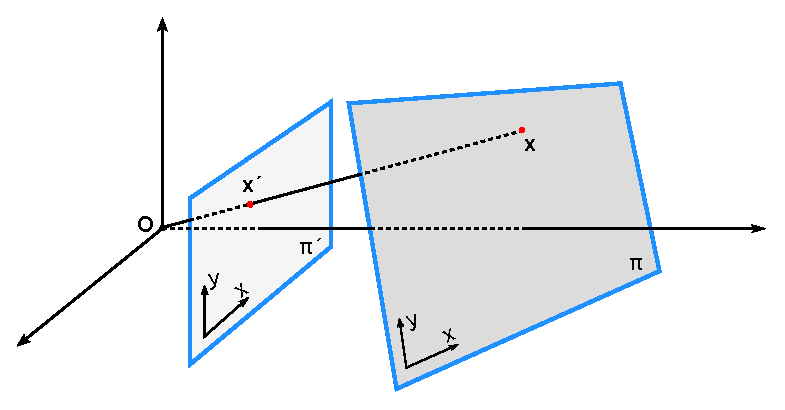
\includegraphics[scale=0.7]{../figs/sizzerman/homografia_esquema}%
\lthtmlpictureZ
\lthtmlcheckvsize\clearpage}

{\newpage\clearpage
\lthtmlinlinemathA{tex2html_wrap_indisplay13243}%
$\displaystyle \begin{bmatrix} sx'_i \\sy'_i\\s   \end{bmatrix}=\textit{H}   \begin{bmatrix}   x_i\\y_i\\1   \end{bmatrix}.$%
\lthtmlindisplaymathZ
\lthtmlcheckvsize\clearpage}

\stepcounter{subsubsection}
\stepcounter{paragraph}
{\newpage\clearpage
\lthtmlinlinemathA{tex2html_wrap_inline13257}%
$ \mathbf{x_{\textrm{i}}\leftrightarrow x_{\textrm{i}}^{\textrm{\ensuremath{\prime}}}}$%
\lthtmlinlinemathZ
\lthtmlcheckvsize\clearpage}

{\newpage\clearpage
\lthtmlinlinemathA{tex2html_wrap_inline13259}%
$ \mathbf{x_{\textrm{i}}^{\textrm{\ensuremath{\prime}}}=\textrm{\textit{H}}x_{\textrm{i}}}$%
\lthtmlinlinemathZ
\lthtmlcheckvsize\clearpage}

{\newpage\clearpage
\lthtmlinlinemathA{tex2html_wrap_inline13261}%
$ \mathbf{x_{\textrm{i}}^{\textrm{\ensuremath{\prime}}}}$%
\lthtmlinlinemathZ
\lthtmlcheckvsize\clearpage}

{\newpage\clearpage
\lthtmlinlinemathA{tex2html_wrap_inline13263}%
$ \mathbf{\textrm{\textit{H}}x_{\textrm{i}}}$%
\lthtmlinlinemathZ
\lthtmlcheckvsize\clearpage}

{\newpage\clearpage
\lthtmlinlinemathA{tex2html_wrap_inline13265}%
$ \mathbf{x_{\textrm{i}}=}(x_{i},y_{i},w_{i})^{\mathsf{T}}$%
\lthtmlinlinemathZ
\lthtmlcheckvsize\clearpage}

{\newpage\clearpage
\lthtmlinlinemathA{tex2html_wrap_inline13267}%
$ \mathbf{x_{\textrm{i}}^{\prime}=}(x_{i}^{\prime},y_{i}^{\prime},w_{i}^{\prime})^{\mathsf{T}}$%
\lthtmlinlinemathZ
\lthtmlcheckvsize\clearpage}

{\newpage\clearpage
\lthtmlinlinemathA{tex2html_wrap_inline13269}%
$ \textit{H}=\left(\begin{array}{c}
\mathbf{\mathbf{h^{\textrm{1}\mathsf{T}}}}\\
\mathbf{h}^{\textrm{2}\textsf{T}}\\
\mathbf{h}^{\textrm{3}\textsf{T}}
\end{array}\right)$%
\lthtmlinlinemathZ
\lthtmlcheckvsize\clearpage}

{\newpage\clearpage
\lthtmlinlinemathA{tex2html_wrap_inline13271}%
$ \mathbf{h^{\textrm{i}\textsf{T}}}$%
\lthtmlinlinemathZ
\lthtmlcheckvsize\clearpage}

{\newpage\clearpage
\lthtmlinlinemathA{tex2html_wrap_inline13273}%
$ i$%
\lthtmlinlinemathZ
\lthtmlcheckvsize\clearpage}

{\newpage\clearpage
\lthtmlinlinemathA{tex2html_wrap_indisplay13279}%
$\displaystyle \begin{bmatrix}\mathbf{0}^{\textsf{T}} & -w_{i}^{\prime}\mathbf{x_{\textrm{i}}^{\textrm{\textsf{T}}}} & y_{i}^{\prime}\mathbf{x_{\textrm{i}}^{\textrm{\textsf{T}}}}\\w_{i}^{\prime}\mathbf{x_{\textrm{i}}^{\textrm{\textsf{T}}}} & \mathbf{0}^{\textsf{T}} & -x_{i}^{\prime}\mathbf{x_{\textrm{i}}^{\textrm{\textsf{T}}}} \end{bmatrix}\begin{pmatrix}\mathbf{h^{\textrm{1}}}\\\mathbf{h^{\textrm{2}}}\\\mathbf{h^{\textrm{3}}} \end{pmatrix}=\mathbf{0}.$%
\lthtmlindisplaymathZ
\lthtmlcheckvsize\clearpage}

{\newpage\clearpage
\lthtmlinlinemathA{tex2html_wrap_inline13281}%
$ A_{i} \mathbf{h}=\mathbf{0}$%
\lthtmlinlinemathZ
\lthtmlcheckvsize\clearpage}

{\newpage\clearpage
\lthtmlinlinemathA{tex2html_wrap_inline13283}%
$ A_{i}$%
\lthtmlinlinemathZ
\lthtmlcheckvsize\clearpage}

{\newpage\clearpage
\lthtmlinlinemathA{tex2html_wrap_inline13287}%
$ \mathbf{h}$%
\lthtmlinlinemathZ
\lthtmlcheckvsize\clearpage}

{\newpage\clearpage
\lthtmlinlinemathA{tex2html_wrap_inline13289}%
$ 9 \times 1$%
\lthtmlinlinemathZ
\lthtmlcheckvsize\clearpage}

{\newpage\clearpage
\lthtmlinlinemathA{tex2html_wrap_inline13291}%
$ 8 \times 8$%
\lthtmlinlinemathZ
\lthtmlcheckvsize\clearpage}

{\newpage\clearpage
\lthtmlinlinemathA{tex2html_wrap_inline13297}%
$ A\mathbf{h}=\mathbf{0}$%
\lthtmlinlinemathZ
\lthtmlcheckvsize\clearpage}

{\newpage\clearpage
\lthtmlinlinemathA{tex2html_wrap_inline13299}%
$ 50\%$%
\lthtmlinlinemathZ
\lthtmlcheckvsize\clearpage}

\stepcounter{paragraph}
{\newpage\clearpage
\lthtmlinlinemathA{tex2html_wrap_inline13302}%
$ x'=ax+b$%
\lthtmlinlinemathZ
\lthtmlcheckvsize\clearpage}

{\newpage\clearpage
\lthtmlinlinemathA{tex2html_wrap_inline13304}%
$ t$%
\lthtmlinlinemathZ
\lthtmlcheckvsize\clearpage}

{\newpage\clearpage
\lthtmlinlinemathA{tex2html_wrap_inline13306}%
$ <\mathbf{a},\mathbf{b}>$%
\lthtmlinlinemathZ
\lthtmlcheckvsize\clearpage}

{\newpage\clearpage
\lthtmlinlinemathA{tex2html_wrap_inline13308}%
$ <\mathbf{a},\mathbf{d}>$%
\lthtmlinlinemathZ
\lthtmlcheckvsize\clearpage}

{\newpage\clearpage
\lthtmlpictureA{tex2html_wrap13312}%
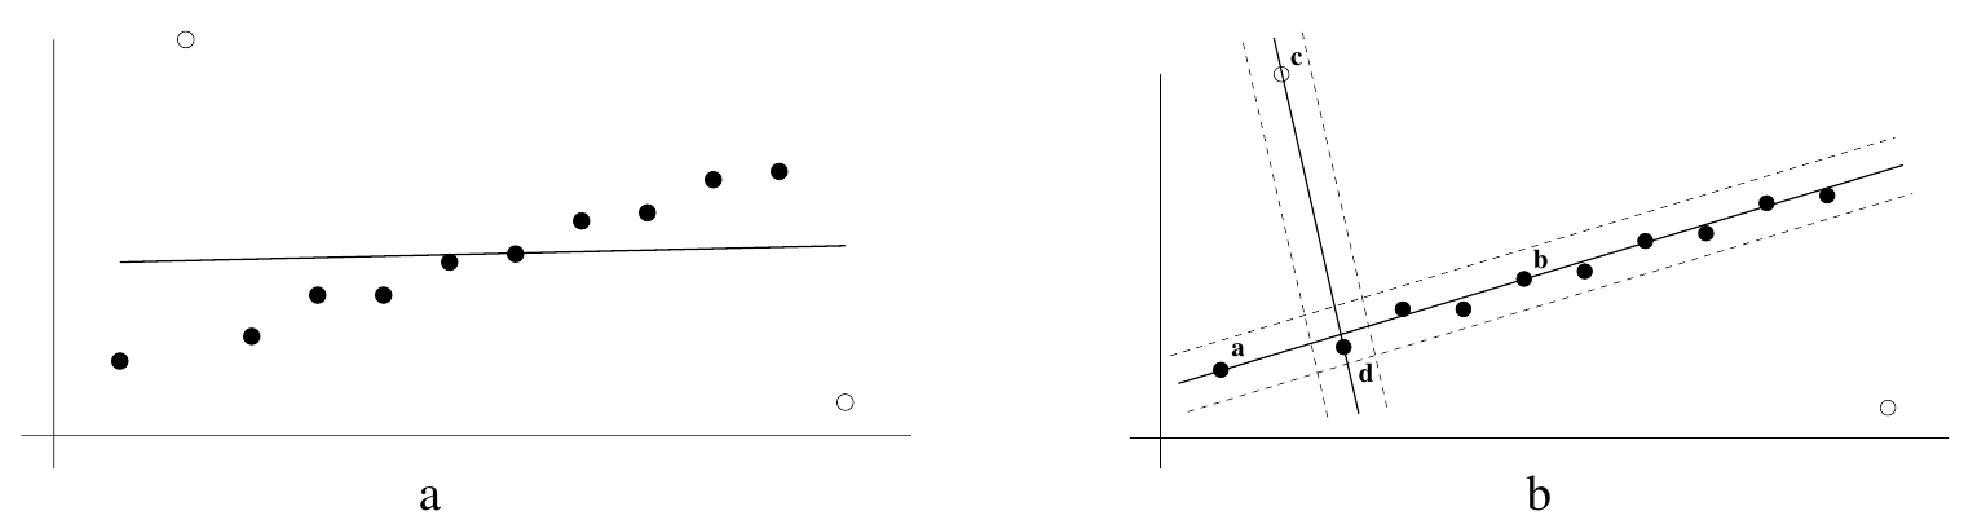
\includegraphics[scale=0.4]{../figs/robust_line_estimation}%
\lthtmlpictureZ
\lthtmlcheckvsize\clearpage}

{\newpage\clearpage
\lthtmlinlinemathA{tex2html_wrap_inline13317}%
$ S$%
\lthtmlinlinemathZ
\lthtmlcheckvsize\clearpage}

{\newpage\clearpage
\lthtmlinlinemathA{tex2html_wrap_inline13320}%
$\textstyle \parbox{365pt}{%
\noindent %\textbf{Eksempel.}
\begin{enumerate}[nolistsep]
 \item Se seleccionan aleatoriamente un conjunto de puntos $s \in S$\  y se instancia el modelo para este subconjunto,
 \item Se determina el conjunto de puntos $S_i$\  que se encuentran dentro de un umbral de distancia $t$\  respecto al modelo. El conjunto $S_i$\  es el conjunto consensuado de muestras y define los valores v\~{A}!`lidos de $S$.
 \item Si la cantidad de elementos v\~{A}!`lidos en $S_i$\  es mayor que un umbral $T$, se estima nuevamente el modelo usando todos los puntos de $S_i$\  y se termina el algoritmo.
 \item Si la cantidad de elementos v\~{A}!`lidos en $S_i$\  es menor que $T$, se selecciona un nuevo subconjunto y se repiten los pasos arriba mencionados.
 \item Luego de $N$\  iteraciones, el conjunto consensuado $S_i$\  con mayor cantidad de elementos es seleccionado y se estima el modelo usando este conjunto de datos.
\end{enumerate}}$%
\lthtmlinlinemathZ
\lthtmlcheckvsize\clearpage}

{\newpage\clearpage
\lthtmlinlinemathA{tex2html_wrap_inline13324}%
$ N$%
\lthtmlinlinemathZ
\lthtmlcheckvsize\clearpage}

{\newpage\clearpage
\lthtmlinlinemathA{tex2html_wrap_inline13330}%
$ {d_{\perp}}^{2}=d(\mathbf{x},\mathbf{\hat{x}})^2+d(\mathbf{x^\prime},\mathbf{\hat{x}^\prime})^2$%
\lthtmlinlinemathZ
\lthtmlcheckvsize\clearpage}

{\newpage\clearpage
\lthtmlinlinemathA{tex2html_wrap_inline13332}%
$ \mathbf{x} \leftrightarrow \mathbf{x^\prime}$%
\lthtmlinlinemathZ
\lthtmlcheckvsize\clearpage}

{\newpage\clearpage
\lthtmlinlinemathA{tex2html_wrap_inline13334}%
$ \mathbf{\hat{x}^\prime}=\textit{H}\mathbf{\hat{x}}$%
\lthtmlinlinemathZ
\lthtmlcheckvsize\clearpage}

{\newpage\clearpage
\lthtmlinlinemathA{tex2html_wrap_inline13336}%
$ {d_{\perp}}^{2}>t^2$%
\lthtmlinlinemathZ
\lthtmlcheckvsize\clearpage}

{\newpage\clearpage
\lthtmlinlinemathA{tex2html_wrap_inline13338}%
$ {d_{\perp}}^{2} \leq t^2$%
\lthtmlinlinemathZ
\lthtmlcheckvsize\clearpage}

{\newpage\clearpage
\lthtmlinlinemathA{tex2html_wrap_inline13346}%
$ 95\%$%
\lthtmlinlinemathZ
\lthtmlcheckvsize\clearpage}

{\newpage\clearpage
\lthtmlinlinemathA{tex2html_wrap_inline13348}%
$ t^2=5.99\sigma^2$%
\lthtmlinlinemathZ
\lthtmlcheckvsize\clearpage}

{\newpage\clearpage
\lthtmlinlinemathA{tex2html_wrap_inline13354}%
$ T=(1-\epsilon)n$%
\lthtmlinlinemathZ
\lthtmlcheckvsize\clearpage}

{\newpage\clearpage
\lthtmlinlinemathA{tex2html_wrap_inline13364}%
$ p=0.99$%
\lthtmlinlinemathZ
\lthtmlcheckvsize\clearpage}

{\newpage\clearpage
\lthtmlinlinemathA{tex2html_wrap_inline13368}%
$ \epsilon=1-w$%
\lthtmlinlinemathZ
\lthtmlcheckvsize\clearpage}

{\newpage\clearpage
\lthtmlinlinemathA{tex2html_wrap_inline13374}%
$ (1-w^s)^{N}=1-p$%
\lthtmlinlinemathZ
\lthtmlcheckvsize\clearpage}

{\newpage\clearpage
\lthtmlinlinemathA{tex2html_wrap_indisplay13378}%
$\displaystyle N=\log(1-p)/\log{(1-(1-\epsilon)^s)}.$%
\lthtmlindisplaymathZ
\lthtmlcheckvsize\clearpage}

{\newpage\clearpage
\lthtmlinlinemathA{tex2html_wrap_inline13380}%
$ s=4$%
\lthtmlinlinemathZ
\lthtmlcheckvsize\clearpage}

{\newpage\clearpage
\lthtmlinlinemathA{tex2html_wrap_inline13382}%
$ \epsilon=50\%$%
\lthtmlinlinemathZ
\lthtmlcheckvsize\clearpage}

{\newpage\clearpage
\lthtmlinlinemathA{tex2html_wrap_inline13386}%
$ \epsilon$%
\lthtmlinlinemathZ
\lthtmlcheckvsize\clearpage}

\stepcounter{subparagraph}
{\newpage\clearpage
\lthtmlinlinemathA{tex2html_wrap_inline13395}%
$ \epsilon=0.5$%
\lthtmlinlinemathZ
\lthtmlcheckvsize\clearpage}

{\newpage\clearpage
\lthtmlinlinemathA{tex2html_wrap_inline13397}%
$ 80\%$%
\lthtmlinlinemathZ
\lthtmlcheckvsize\clearpage}

{\newpage\clearpage
\lthtmlinlinemathA{tex2html_wrap_inline13399}%
$ \epsilon=0.2$%
\lthtmlinlinemathZ
\lthtmlcheckvsize\clearpage}

{\newpage\clearpage
\lthtmlinlinemathA{tex2html_wrap_inline13418}%
$\textstyle \parbox{365pt}{%
\noindent %\textbf{Eksempel.}
\begin{enumerate}[nolistsep]
 \item $N=\infty$, $contador\_muestras=0$.
 \item Mientras $N>contador\_muestras$\  repetir:
  \begin{itemize}
    \item Seleccionar una muestra y contar el n\~{A}\ensuremath{^{o}}mero de valores v\~{A}!`lidos. 
    \item Establecer $\epsilon=1-\frac{\text{cantidad de valores v\~{A}!`lidos}}{\text{cantidad total de puntos}}$
    \item Establecer $N$\  con $\epsilon$\  seg\~{A}\ensuremath{^{o}}n la ecuaci\~{A}\ensuremath{^{3}}n \eqref{eq:determineN} para $p=0.99$
    \item Incrementar $contador\_muestras$\  por 1
  \end{itemize}
 \item Fin.
\end{enumerate}}$%
\lthtmlinlinemathZ
\lthtmlcheckvsize\clearpage}

{\newpage\clearpage
\lthtmlinlinemathA{tex2html_wrap_inline13419}%
$\textstyle \parbox{365pt}{%
\noindent \textbf{C\~{A}!`lculo de la homograf\~{A}\-a 2D entre dos im\~{A}!`genes.}
\begin{enumerate}[nolistsep]
 \item Se asume que se tiene un conjunto de potenciales correspondencias entre las im\~{A}!`genes.
 \item Se repite para $N$\  muestras ($N$\  determinado con el algoritmo adaptativo)
  \begin{itemize}
    \item Se seleccionan aleatoriamente cuatro correspondencias y se calcula la homograf\~{A}\-a $\textit{H}$.
    \item Se calcula la distancia $d_{\perp}$\  para cada correspondencia.
    \item Se calcula la cantidad de valores v\~{A}!`lidos consistentes con $\textit{H}$\  entre la cantidad de correspondencias para las cuales $d_{\perp}<t=\sqrt{5.99}\sigma$\  p\~{A}\-xeles.
  \end{itemize}
  Seleccionar $\textit{H}$\  con la mayor cantidad de valores v\~{A}!`lidos. 
 \item Re-estimar $\textit{H}$\  a partir de todas las correspondencias clasificadas como v\~{A}!`lidas, mediante la minimizaci\~{A}\ensuremath{^{3}}n de la funci\~{A}\ensuremath{^{3}}n acumulada de error de reproyecci\~{A}\ensuremath{^{3}}n: $\underset{i}{\sum}d(\mathbf{x}_{i},\hat{\mathbf{x}}_{i})^{2}+d(\mathbf{x}_{i}^{\prime},\hat{\mathbf{x}}_{i}^{\prime})^{2}$\  sujeto a $\hat{\mathbf{x}}_{i}^\prime=\hat{\textit{H}}\hat{\mathbf{x}_i}\; \forall i$\  usando el algoritmo de Levenberg-Marquardt.
\end{enumerate}}$%
\lthtmlinlinemathZ
\lthtmlcheckvsize\clearpage}

\stepcounter{chapter}
\stepcounter{section}
{\newpage\clearpage
\lthtmlpictureA{tex2html_wrap13425}%
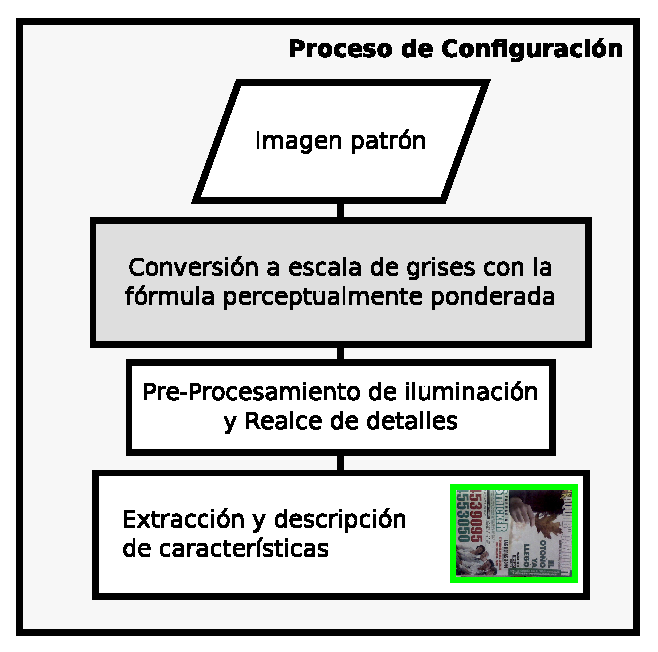
\includegraphics[scale=0.7]{../figs/proceso_completo_entrenamiento}%
\lthtmlpictureZ
\lthtmlcheckvsize\clearpage}

{\newpage\clearpage
\lthtmlpictureA{tex2html_wrap13429}%
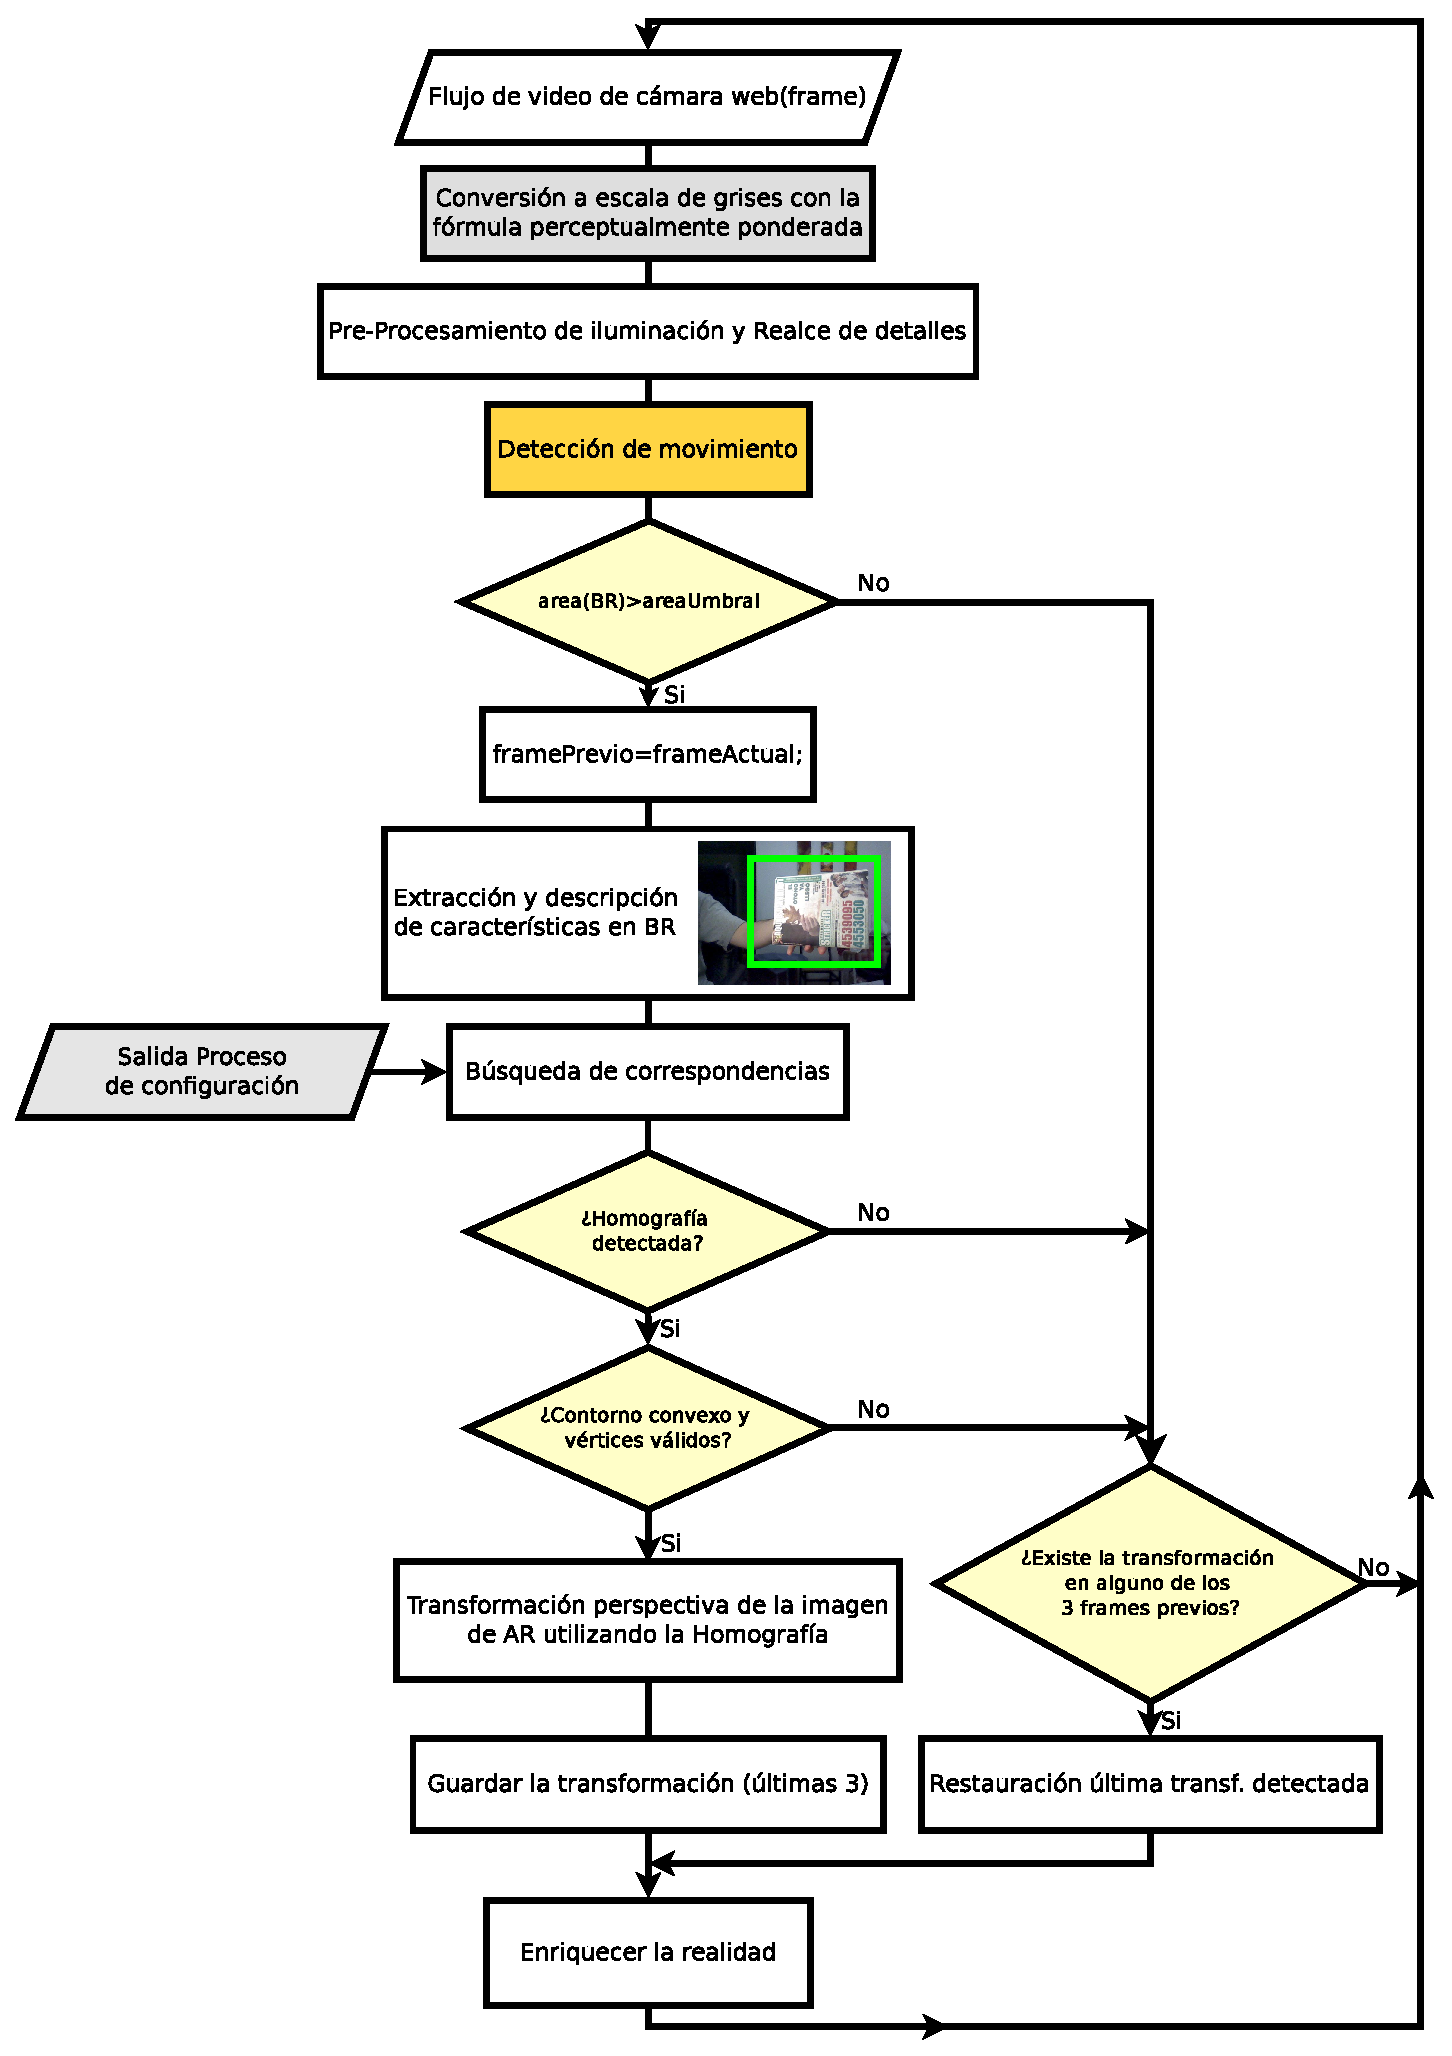
\includegraphics[scale=0.57]{../figs/proceso_completo}%
\lthtmlpictureZ
\lthtmlcheckvsize\clearpage}

\stepcounter{section}
{\newpage\clearpage
\lthtmlinlinemathA{tex2html_wrap_inline13435}%
$ G$%
\lthtmlinlinemathZ
\lthtmlcheckvsize\clearpage}

{\newpage\clearpage
\lthtmlinlinemathA{tex2html_wrap_indisplay13441}%
$\displaystyle I=0.299R+0.587G+0.114B.$%
\lthtmlindisplaymathZ
\lthtmlcheckvsize\clearpage}

\stepcounter{section}
\stepcounter{section}
{\newpage\clearpage
\lthtmlpictureA{tex2html_wrap13447}%
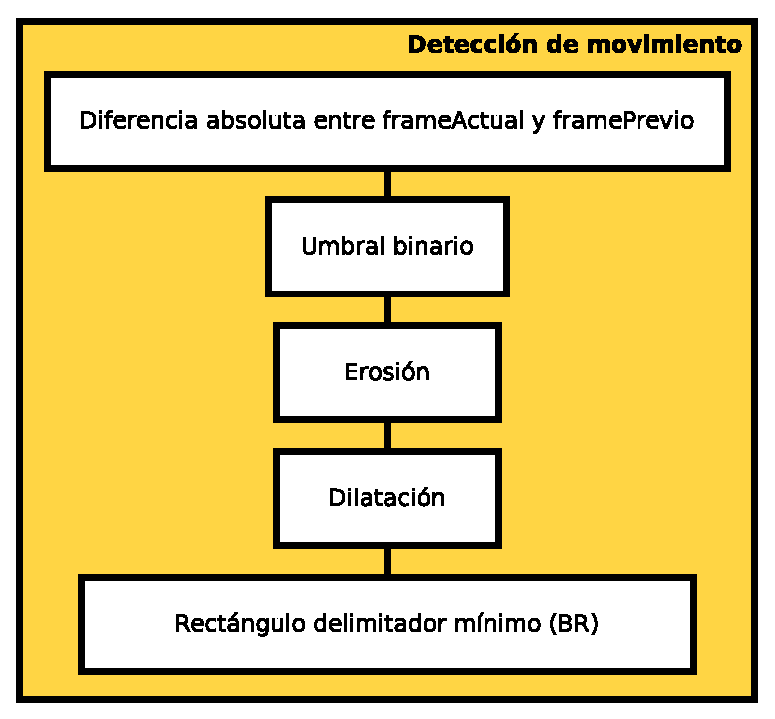
\includegraphics[scale=0.65]{../figs/procesomovimiento}%
\lthtmlpictureZ
\lthtmlcheckvsize\clearpage}

{\newpage\clearpage
\lthtmlpictureA{tex2html_wrap13448}%
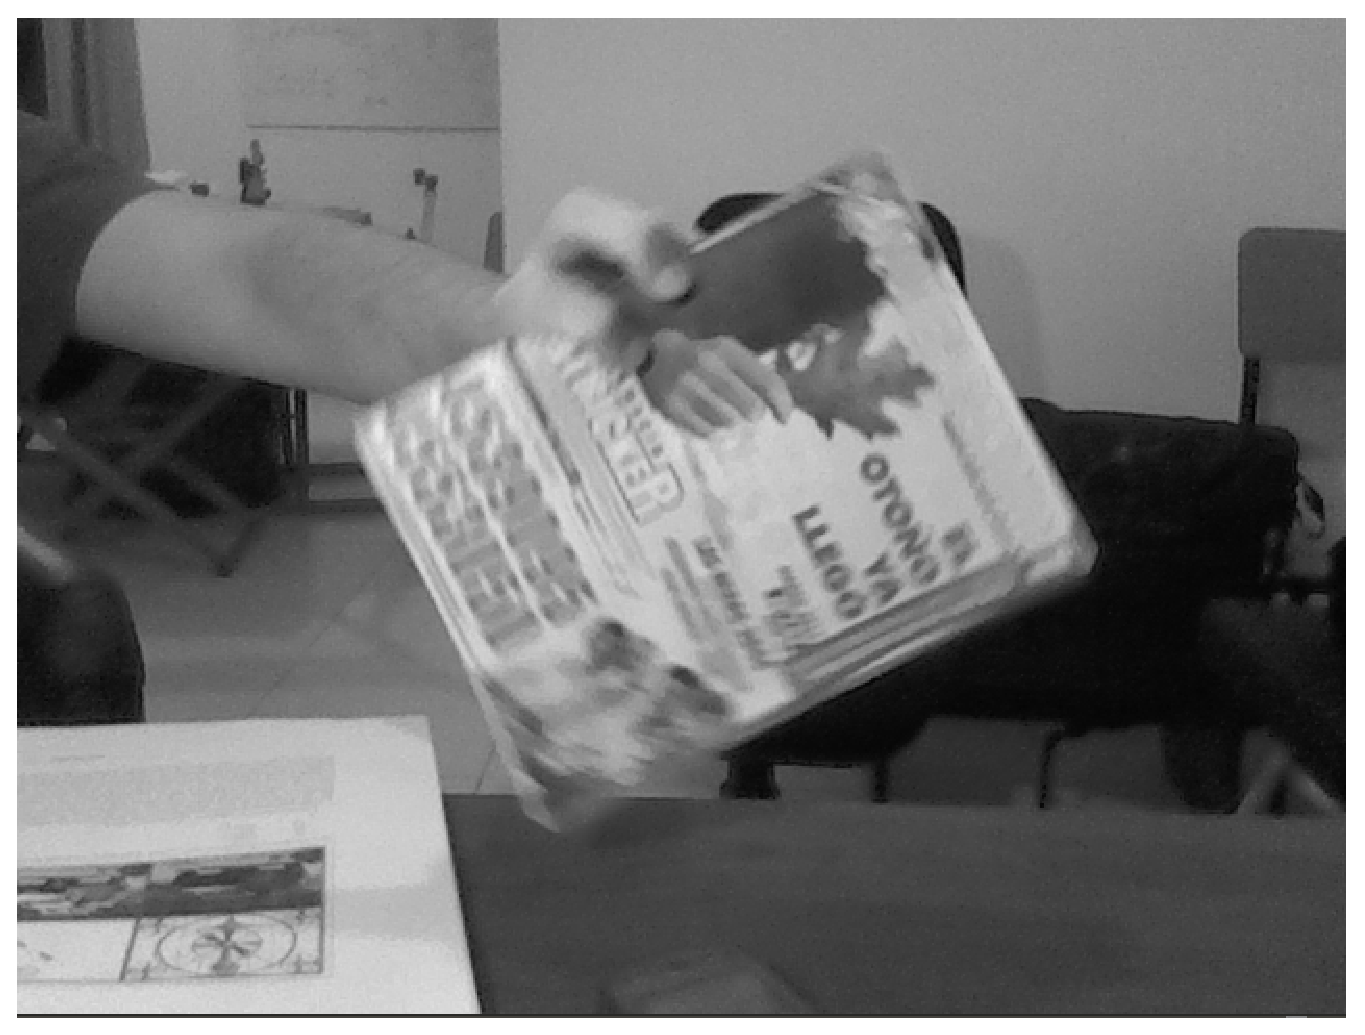
\includegraphics[width=2.3in]{../figs/preprocess/srcPrev}%
\lthtmlpictureZ
\lthtmlcheckvsize\clearpage}

{\newpage\clearpage
\lthtmlpictureA{tex2html_wrap13449}%
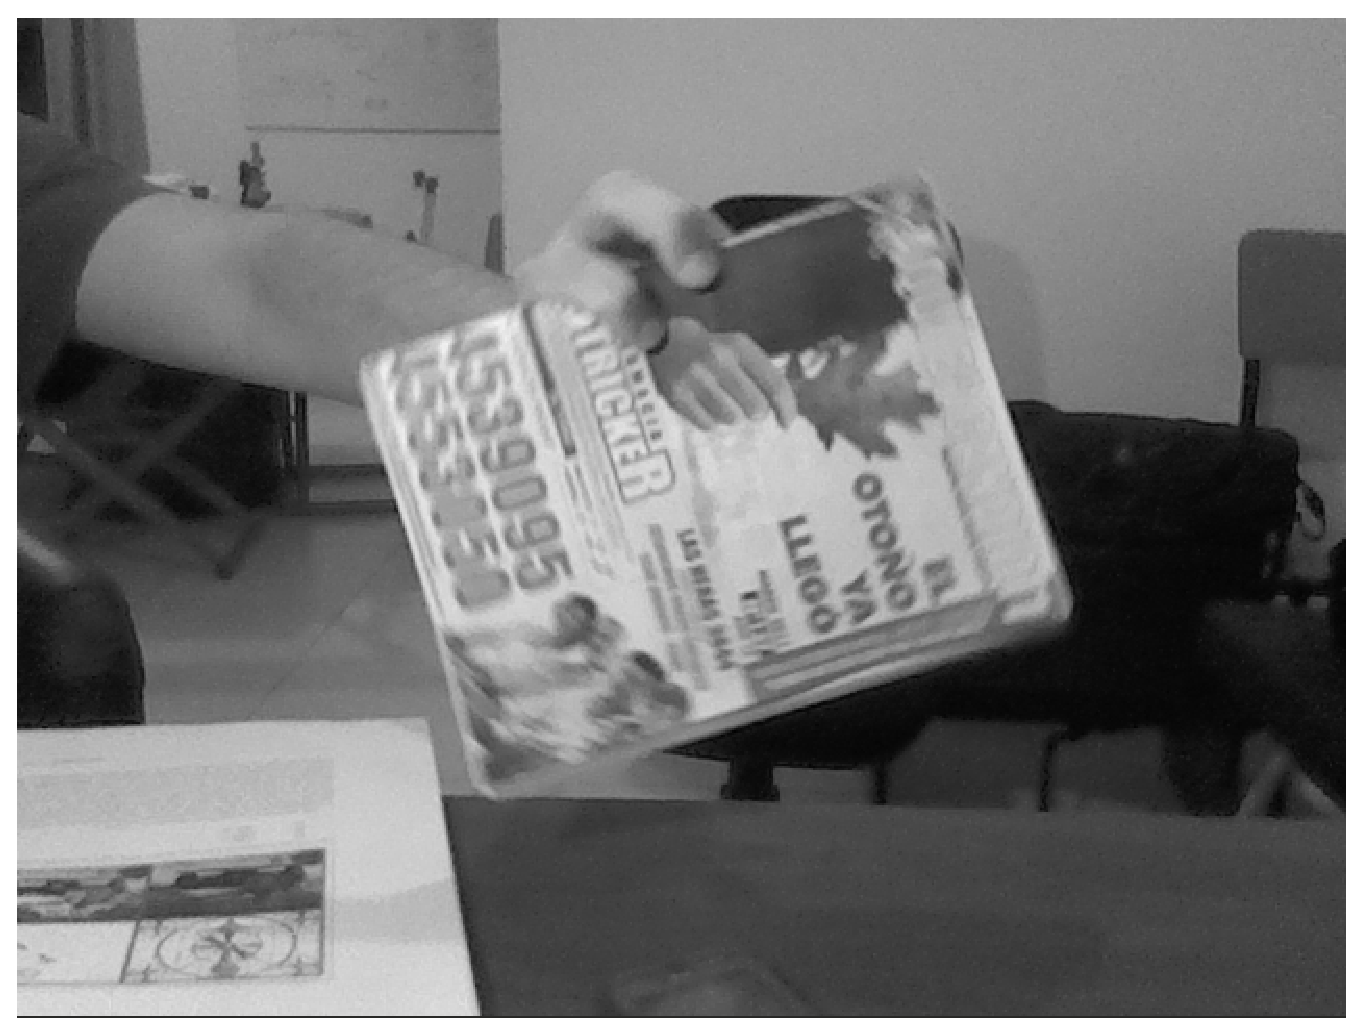
\includegraphics[width=2.3in]{../figs/preprocess/src}%
\lthtmlpictureZ
\lthtmlcheckvsize\clearpage}

{\newpage\clearpage
\lthtmlpictureA{tex2html_wrap13450}%
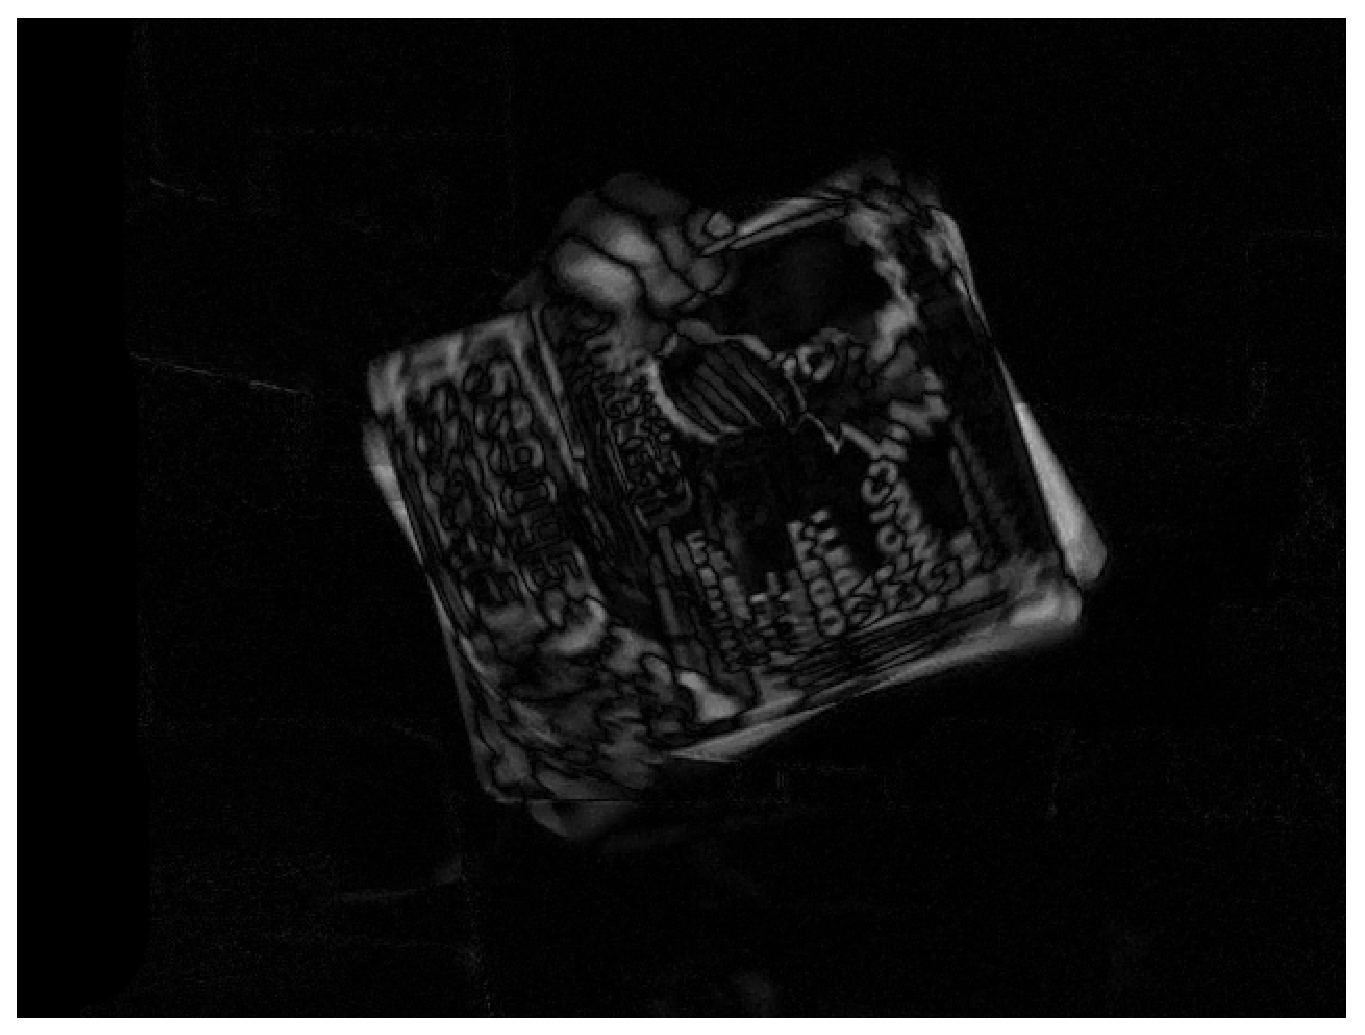
\includegraphics[width=2.3in]{../figs/preprocess/absDiff}%
\lthtmlpictureZ
\lthtmlcheckvsize\clearpage}

{\newpage\clearpage
\lthtmlpictureA{tex2html_wrap13451}%
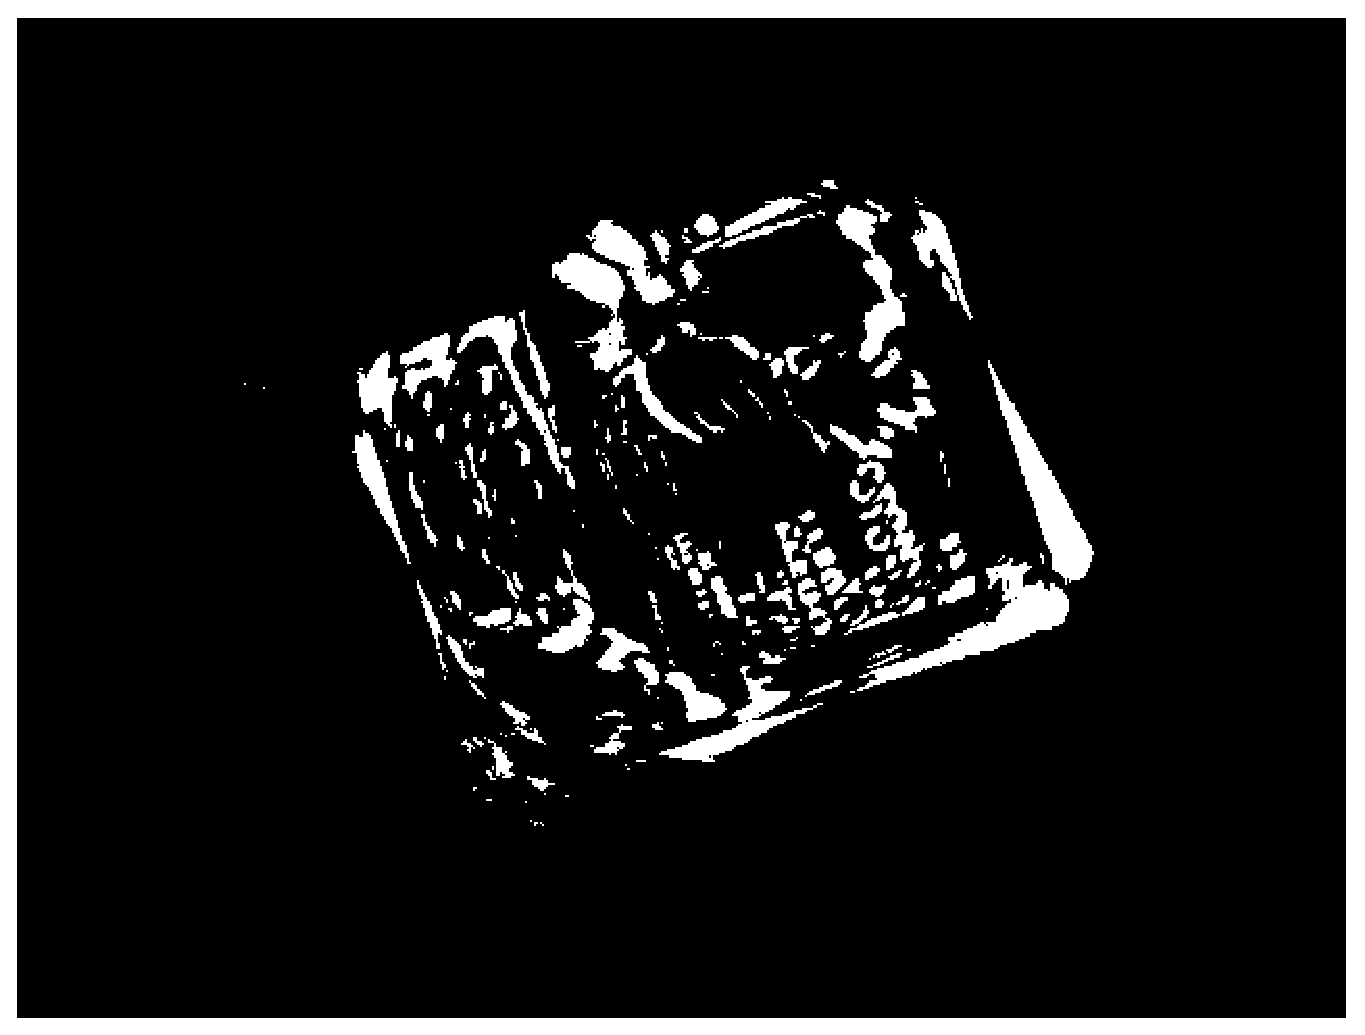
\includegraphics[width=2.3in]{../figs/preprocess/threshold}%
\lthtmlpictureZ
\lthtmlcheckvsize\clearpage}

{\newpage\clearpage
\lthtmlpictureA{tex2html_wrap13454}%
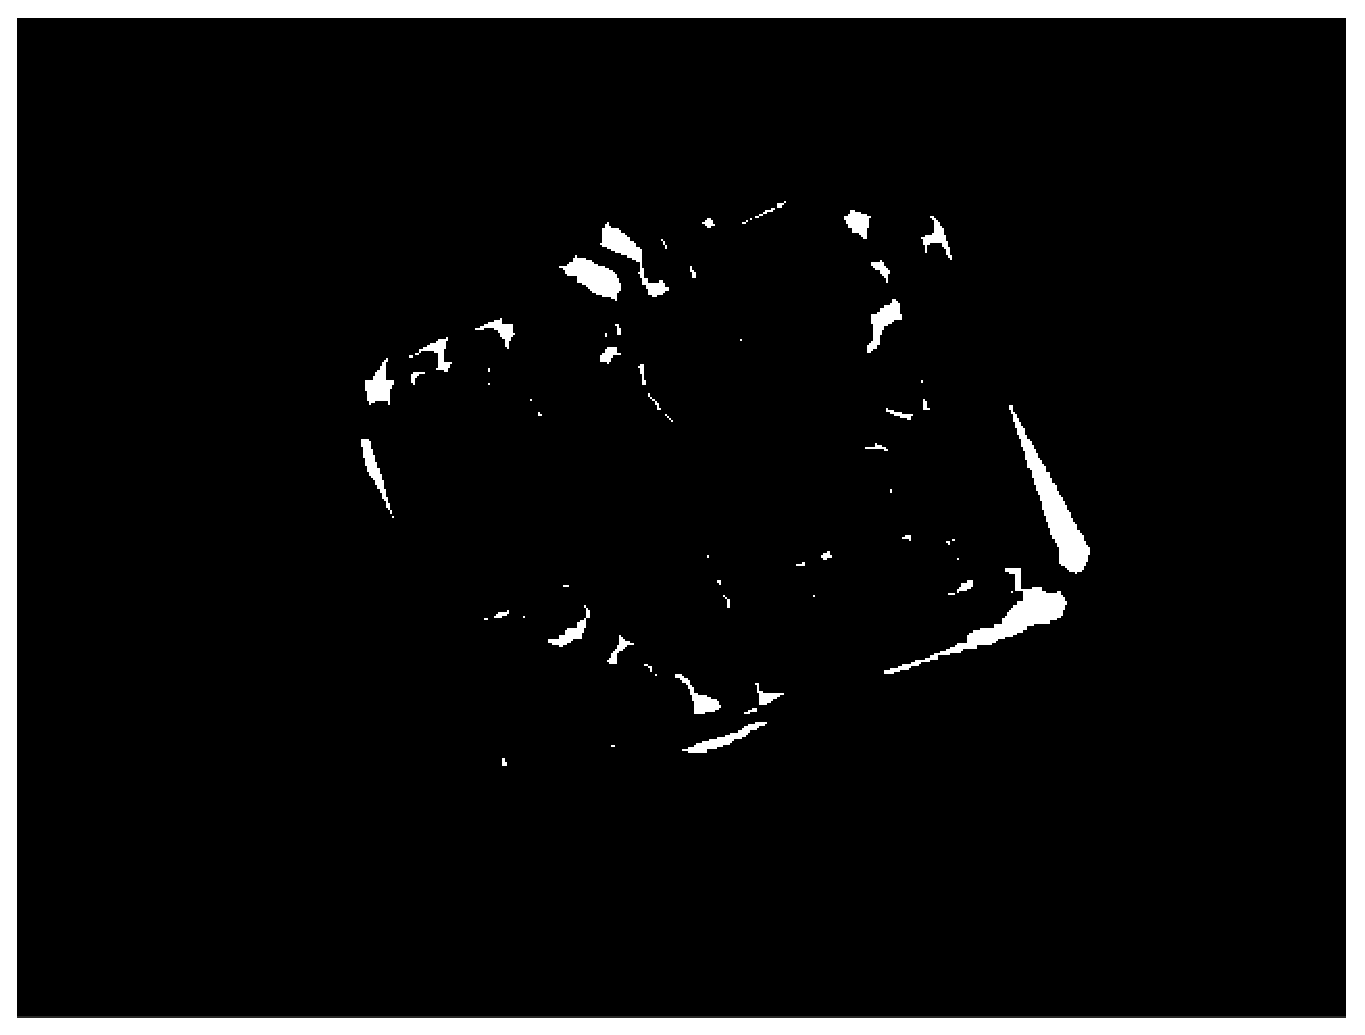
\includegraphics[width=2.3in]{../figs/preprocess/erode}%
\lthtmlpictureZ
\lthtmlcheckvsize\clearpage}

{\newpage\clearpage
\lthtmlpictureA{tex2html_wrap13457}%
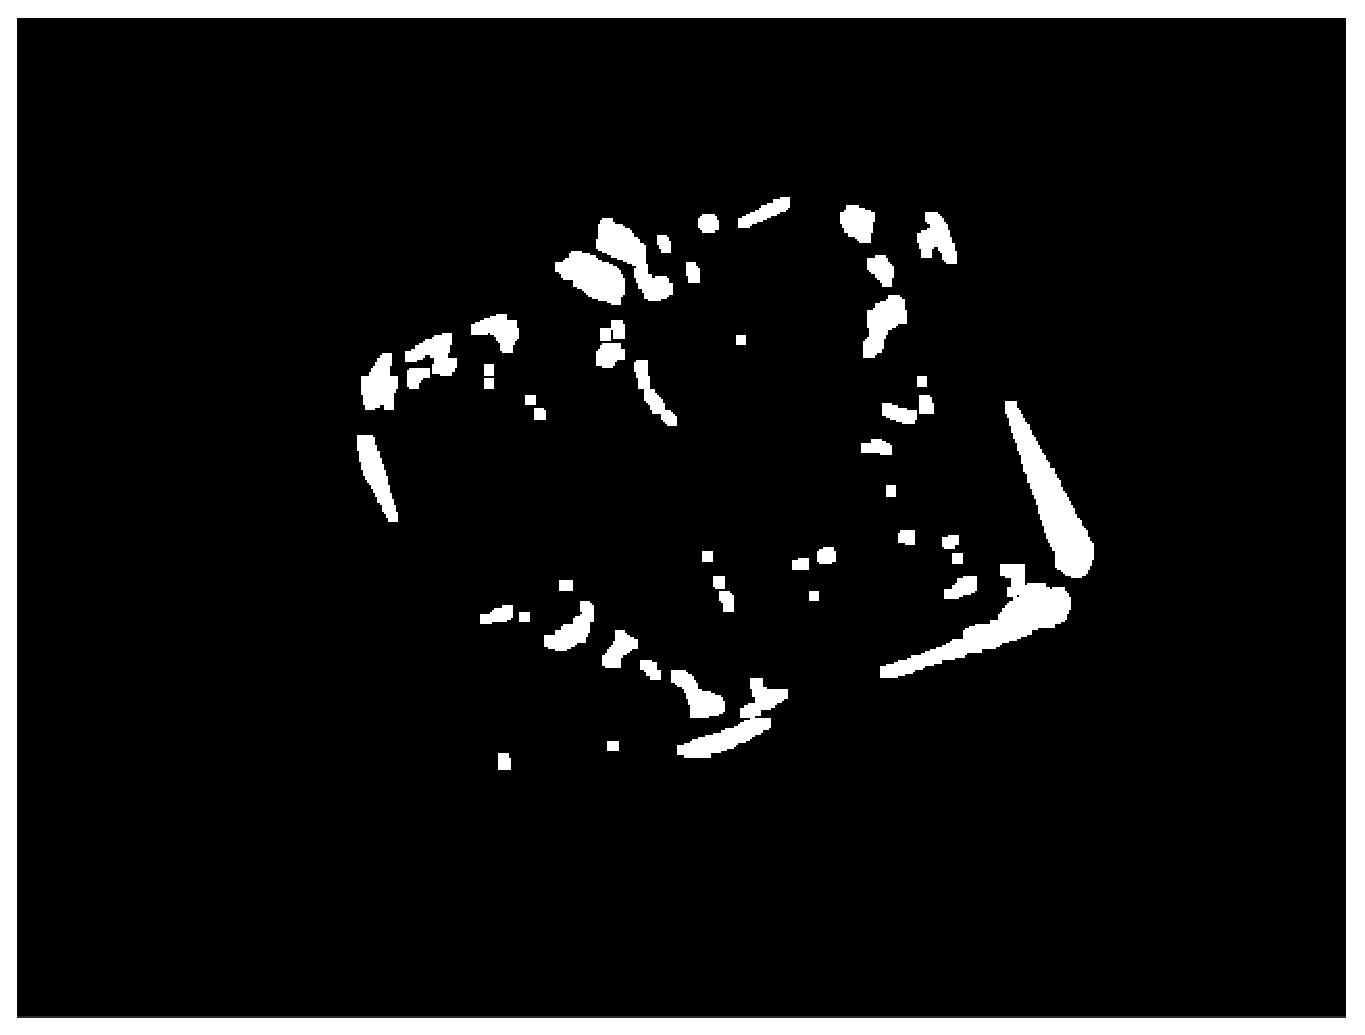
\includegraphics[width=2.3in]{../figs/preprocess/dilate}%
\lthtmlpictureZ
\lthtmlcheckvsize\clearpage}

{\newpage\clearpage
\lthtmlpictureA{tex2html_wrap13458}%
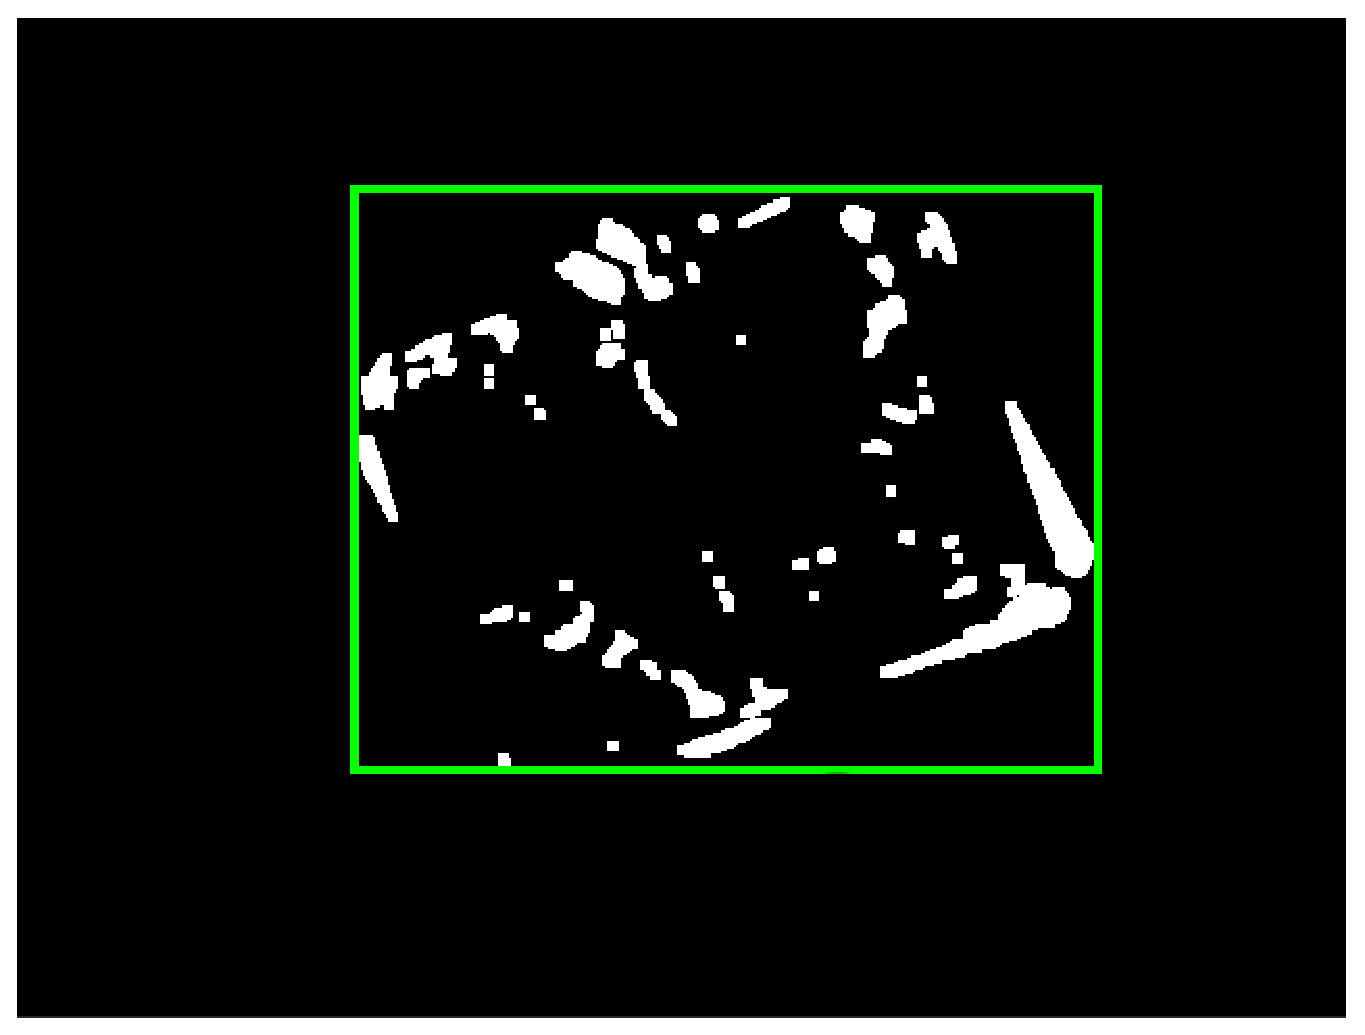
\includegraphics[width=2.3in]{../figs/preprocess/boundingrect}%
\lthtmlpictureZ
\lthtmlcheckvsize\clearpage}

\stepcounter{subsubsection}
{\newpage\clearpage
\lthtmlinlinemathA{tex2html_wrap_inline13464}%
$ F$%
\lthtmlinlinemathZ
\lthtmlcheckvsize\clearpage}

{\newpage\clearpage
\lthtmlinlinemathA{tex2html_wrap_inline13468}%
$ t-1$%
\lthtmlinlinemathZ
\lthtmlcheckvsize\clearpage}

{\newpage\clearpage
\lthtmlinlinemathA{tex2html_wrap_indisplay13470}%
$\displaystyle D(x,y)=|F_{t}(x,y)-F_{t-1}(x,y)|\;\forall\; x,y\;\in F.$%
\lthtmlindisplaymathZ
\lthtmlcheckvsize\clearpage}

{\newpage\clearpage
\lthtmlinlinemathA{tex2html_wrap_inline13474}%
$ framePrevio=frameActual$%
\lthtmlinlinemathZ
\lthtmlcheckvsize\clearpage}

{\newpage\clearpage
\lthtmlinlinemathA{tex2html_wrap_inline13476}%
$ area(BR)>areaUmbral$%
\lthtmlinlinemathZ
\lthtmlcheckvsize\clearpage}

\stepcounter{subsubsection}
{\newpage\clearpage
\lthtmlinlinemathA{tex2html_wrap_inline13481}%
$ s_{max}=255$%
\lthtmlinlinemathZ
\lthtmlcheckvsize\clearpage}

{\newpage\clearpage
\lthtmlinlinemathA{tex2html_wrap_inline13483}%
$ u=50$%
\lthtmlinlinemathZ
\lthtmlcheckvsize\clearpage}

\stepcounter{subsubsection}
\stepcounter{subsubsection}
\stepcounter{subsection}
{\newpage\clearpage
\lthtmlinlinemathA{tex2html_wrap_inline13499}%
$ area(\cdot)$%
\lthtmlinlinemathZ
\lthtmlcheckvsize\clearpage}

{\newpage\clearpage
\lthtmlinlinemathA{tex2html_wrap_inline13501}%
$ areaUmbral$%
\lthtmlinlinemathZ
\lthtmlcheckvsize\clearpage}

{\newpage\clearpage
\lthtmlinlinemathA{tex2html_wrap_inline13503}%
$ BR$%
\lthtmlinlinemathZ
\lthtmlcheckvsize\clearpage}

{\newpage\clearpage
\lthtmlinlinemathA{tex2html_wrap_inline13507}%
$ 10000$%
\lthtmlinlinemathZ
\lthtmlcheckvsize\clearpage}

{\newpage\clearpage
\lthtmlinlinemathA{tex2html_wrap_inline13509}%
$ 100 \times 100$%
\lthtmlinlinemathZ
\lthtmlcheckvsize\clearpage}

{\newpage\clearpage
\lthtmlinlinemathA{tex2html_wrap_inline13511}%
$ 640 \times 480$%
\lthtmlinlinemathZ
\lthtmlcheckvsize\clearpage}

\stepcounter{section}
{\newpage\clearpage
\lthtmlpictureA{tex2html_wrap13513}%
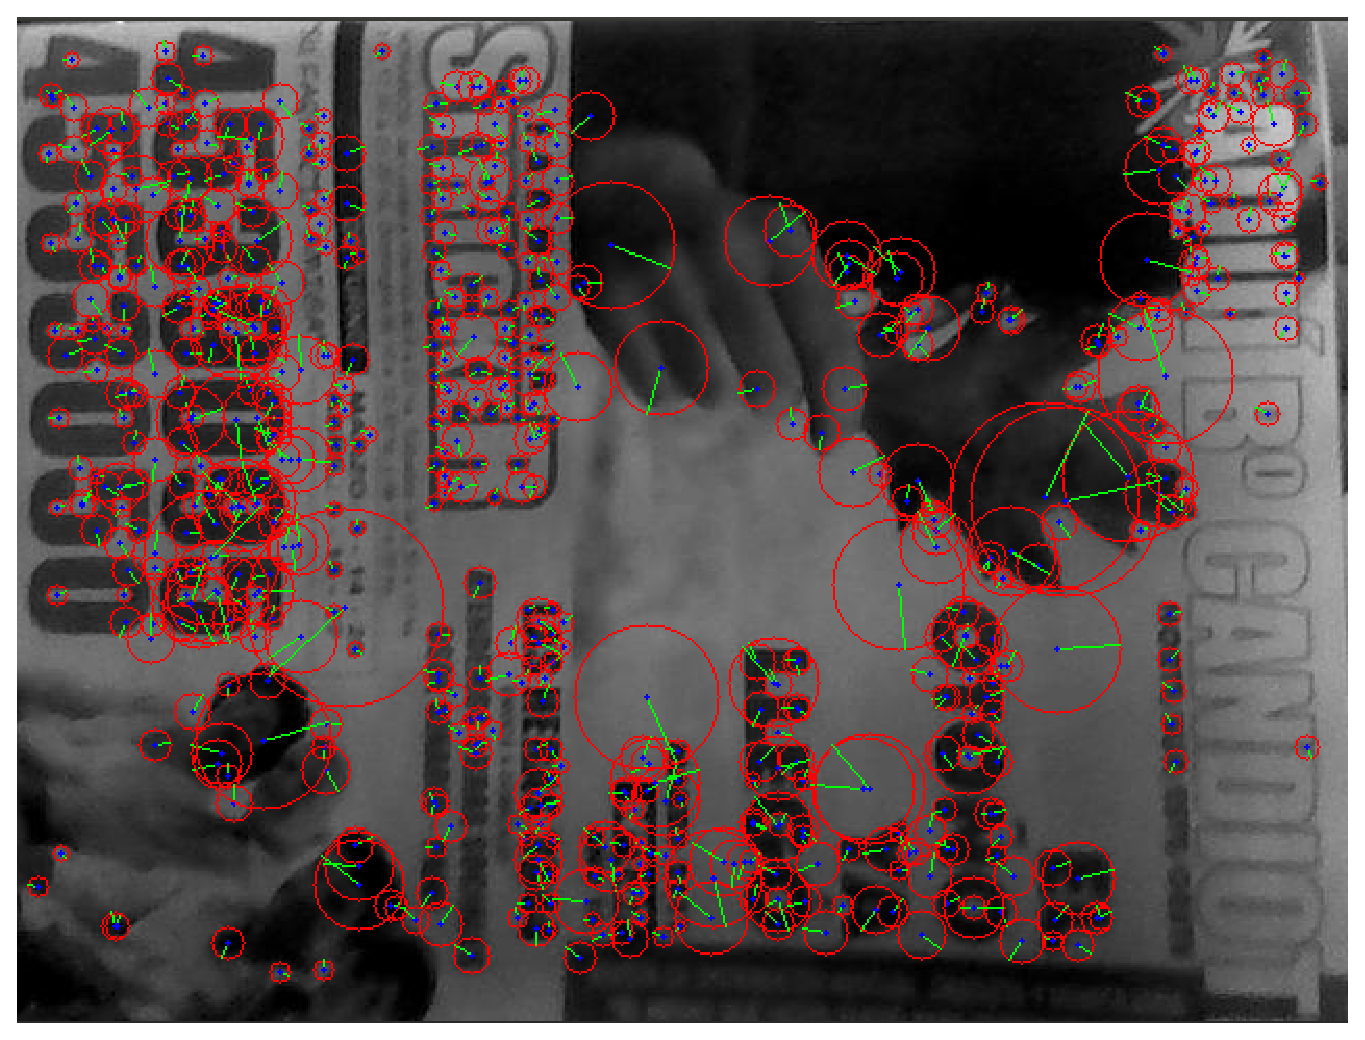
\includegraphics[scale=0.5]{./figs/extraccion/800}%
\lthtmlpictureZ
\lthtmlcheckvsize\clearpage}

{\newpage\clearpage
\lthtmlpictureA{tex2html_wrap13514}%
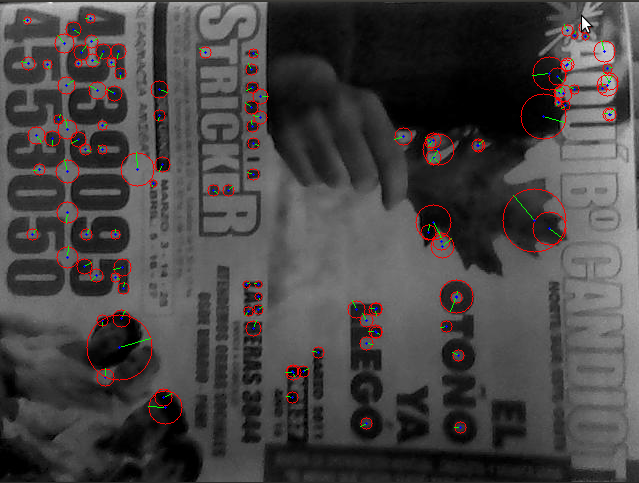
\includegraphics[scale=0.5]{./figs/extraccion/3000}%
\lthtmlpictureZ
\lthtmlcheckvsize\clearpage}

\stepcounter{section}
{\newpage\clearpage
\lthtmlinlinemathA{tex2html_wrap_inline13520}%
$ \mathit{hessianThreshold}=2000$%
\lthtmlinlinemathZ
\lthtmlcheckvsize\clearpage}

{\newpage\clearpage
\lthtmlpictureA{tex2html_wrap13526}%
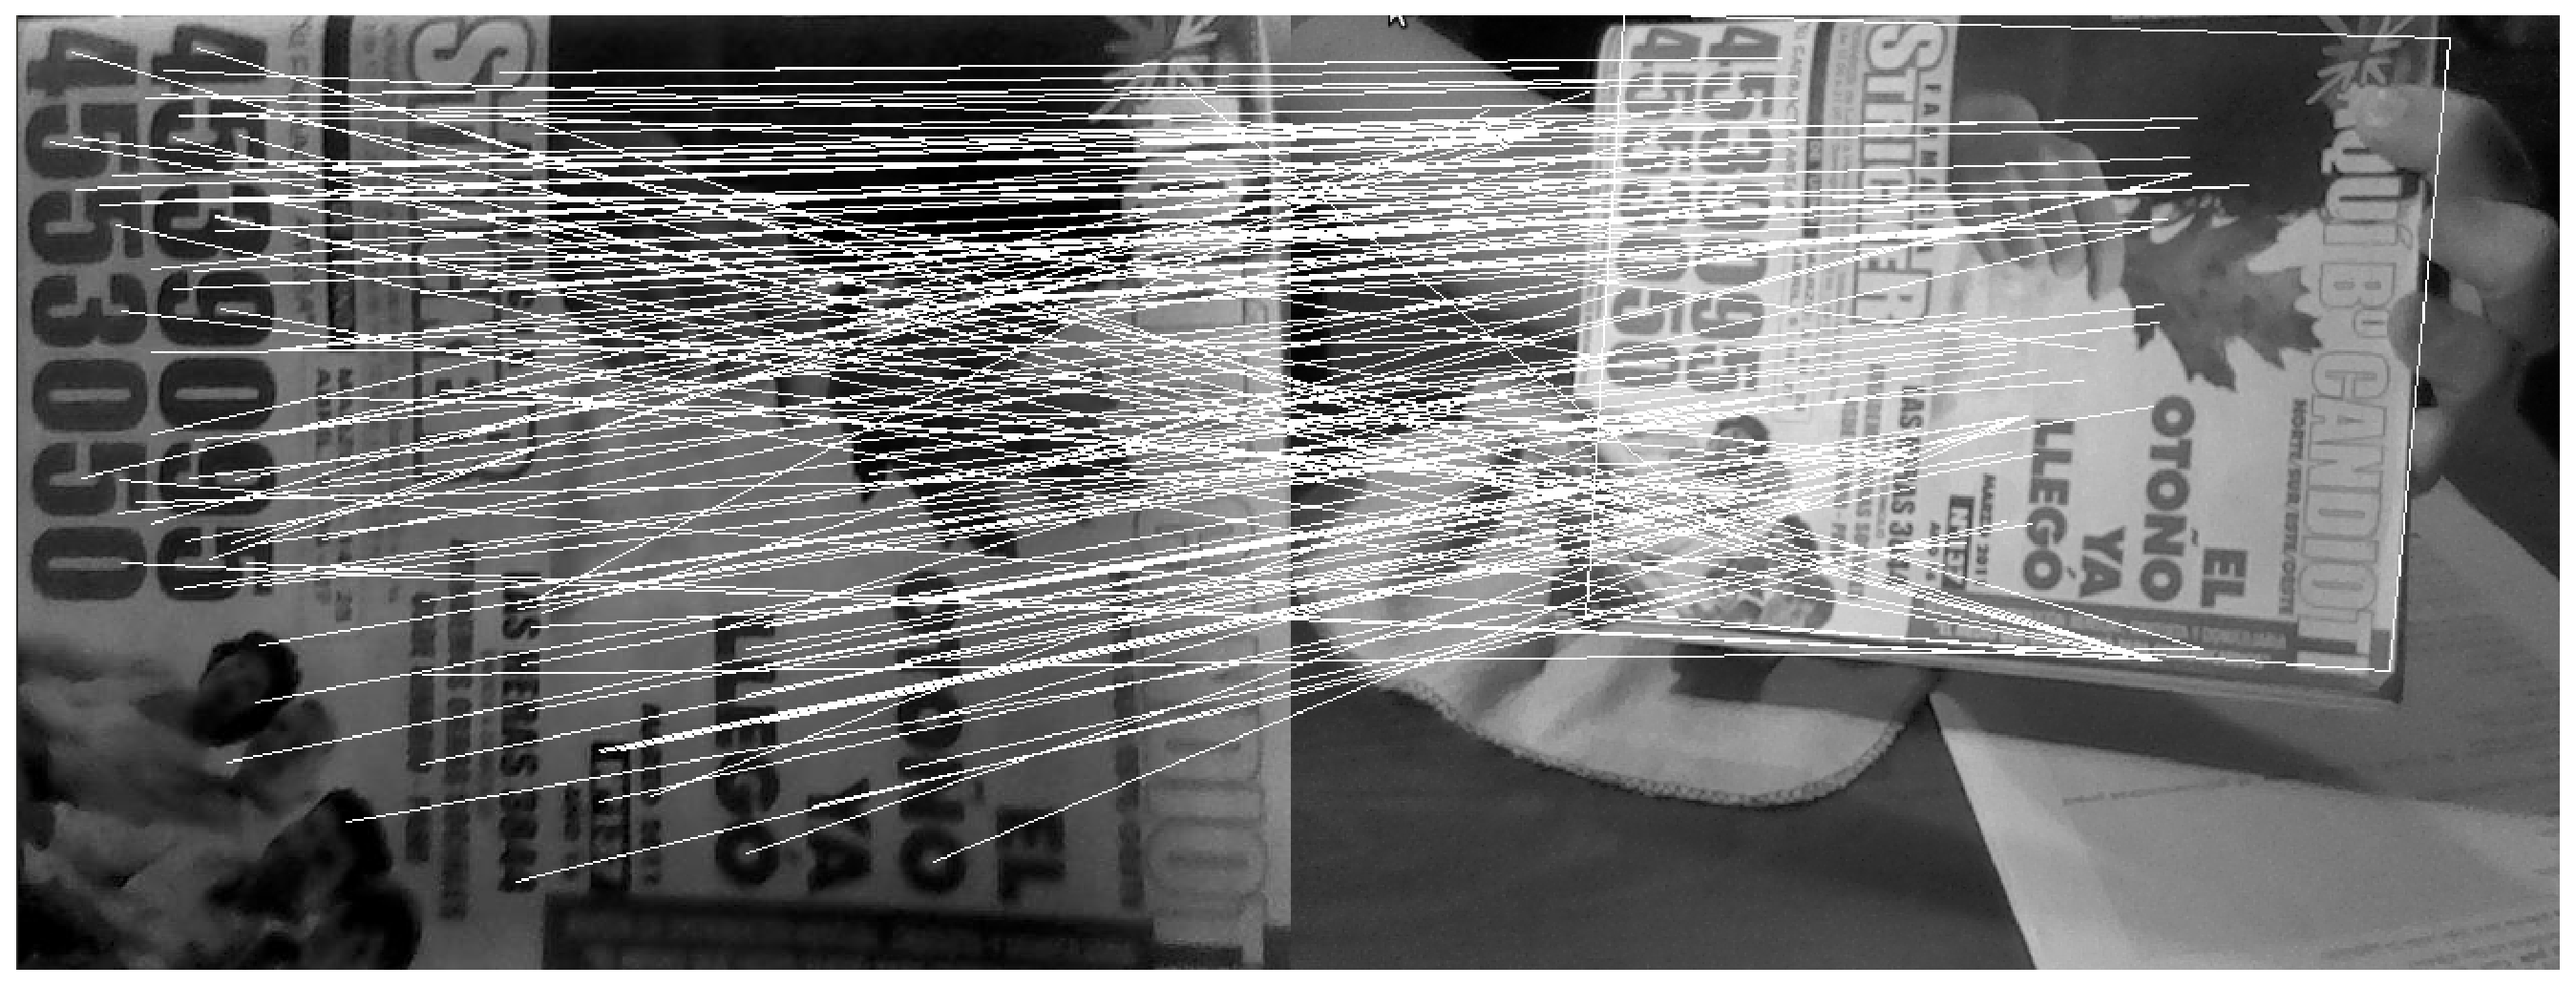
\includegraphics[scale=0.3]{../figs/extraccion/correspondencias}%
\lthtmlpictureZ
\lthtmlcheckvsize\clearpage}

\stepcounter{section}
\stepcounter{section}
\stepcounter{subsubsection}
\stepcounter{subsubsection}
{\newpage\clearpage
\lthtmlinlinemathA{tex2html_wrap_indisplay13534}%
$\displaystyle \resizebox{.8\hsize}{!}{$(| \alpha_x - \gamma_x| < \Delta X) \;\;\vee \;\;(| \beta_x - \lambda_x | < \Delta X) \;\;\vee \;\;| (\alpha_y - \gamma_y | < \Delta Y) \;\;\vee \;\;(|\beta_y - \lambda_y |< \Delta Y),$}$%
\lthtmlindisplaymathZ
\lthtmlcheckvsize\clearpage}

{\newpage\clearpage
\lthtmlinlinemathA{tex2html_wrap_inline13536}%
$ \alpha(x,y)$%
\lthtmlinlinemathZ
\lthtmlcheckvsize\clearpage}

{\newpage\clearpage
\lthtmlinlinemathA{tex2html_wrap_inline13538}%
$ \beta(x,y)$%
\lthtmlinlinemathZ
\lthtmlcheckvsize\clearpage}

{\newpage\clearpage
\lthtmlinlinemathA{tex2html_wrap_inline13540}%
$ \gamma(x,y)$%
\lthtmlinlinemathZ
\lthtmlcheckvsize\clearpage}

{\newpage\clearpage
\lthtmlinlinemathA{tex2html_wrap_inline13542}%
$ \lambda(x,y)$%
\lthtmlinlinemathZ
\lthtmlcheckvsize\clearpage}

{\newpage\clearpage
\lthtmlinlinemathA{tex2html_wrap_inline13544}%
$ \alpha$%
\lthtmlinlinemathZ
\lthtmlcheckvsize\clearpage}

{\newpage\clearpage
\lthtmlinlinemathA{tex2html_wrap_inline13546}%
$ \gamma$%
\lthtmlinlinemathZ
\lthtmlcheckvsize\clearpage}

{\newpage\clearpage
\lthtmlinlinemathA{tex2html_wrap_inline13548}%
$ \beta$%
\lthtmlinlinemathZ
\lthtmlcheckvsize\clearpage}

{\newpage\clearpage
\lthtmlinlinemathA{tex2html_wrap_inline13550}%
$ \lambda$%
\lthtmlinlinemathZ
\lthtmlcheckvsize\clearpage}

{\newpage\clearpage
\lthtmlinlinemathA{tex2html_wrap_inline13556}%
$ \Delta X$%
\lthtmlinlinemathZ
\lthtmlcheckvsize\clearpage}

{\newpage\clearpage
\lthtmlinlinemathA{tex2html_wrap_inline13558}%
$ \Delta Y$%
\lthtmlinlinemathZ
\lthtmlcheckvsize\clearpage}

{\newpage\clearpage
\lthtmlinlinemathA{tex2html_wrap_inline13560}%
$ \Delta X = \Delta Y = 20$%
\lthtmlinlinemathZ
\lthtmlcheckvsize\clearpage}

{\newpage\clearpage
\lthtmlpictureA{tex2html_wrap13561}%
\includegraphics[scale=0.75]{../figs/validaciones_poligono/concavo_invalido}%
\lthtmlpictureZ
\lthtmlcheckvsize\clearpage}

{\newpage\clearpage
\lthtmlpictureA{tex2html_wrap13562}%
\includegraphics[scale=0.75]{../figs/validaciones_poligono/convexo_invalido}%
\lthtmlpictureZ
\lthtmlcheckvsize\clearpage}

{\newpage\clearpage
\lthtmlpictureA{tex2html_wrap13563}%
\includegraphics[scale=0.75]{../figs/validaciones_poligono/poligoto_fuera_viewport_valida}%
\lthtmlpictureZ
\lthtmlcheckvsize\clearpage}

\stepcounter{section}
{\newpage\clearpage
\lthtmlinlinemathA{tex2html_wrap_inline13573}%
$ f_t$%
\lthtmlinlinemathZ
\lthtmlcheckvsize\clearpage}

{\newpage\clearpage
\lthtmlinlinemathA{tex2html_wrap_inline13575}%
$ f_{t-i}$%
\lthtmlinlinemathZ
\lthtmlcheckvsize\clearpage}

{\newpage\clearpage
\lthtmlinlinemathA{tex2html_wrap_inline13577}%
$ i=1,2,3 \ldots n$%
\lthtmlinlinemathZ
\lthtmlcheckvsize\clearpage}

{\newpage\clearpage
\lthtmlinlinemathA{tex2html_wrap_inline13581}%
$ f_{t-2}$%
\lthtmlinlinemathZ
\lthtmlcheckvsize\clearpage}

{\newpage\clearpage
\lthtmlinlinemathA{tex2html_wrap_inline13583}%
$ f_{t-1}$%
\lthtmlinlinemathZ
\lthtmlcheckvsize\clearpage}

{\newpage\clearpage
\lthtmlinlinemathA{tex2html_wrap_inline13585}%
$ f_{t}$%
\lthtmlinlinemathZ
\lthtmlcheckvsize\clearpage}

{\newpage\clearpage
\lthtmlpictureA{tex2html_wrap13589}%
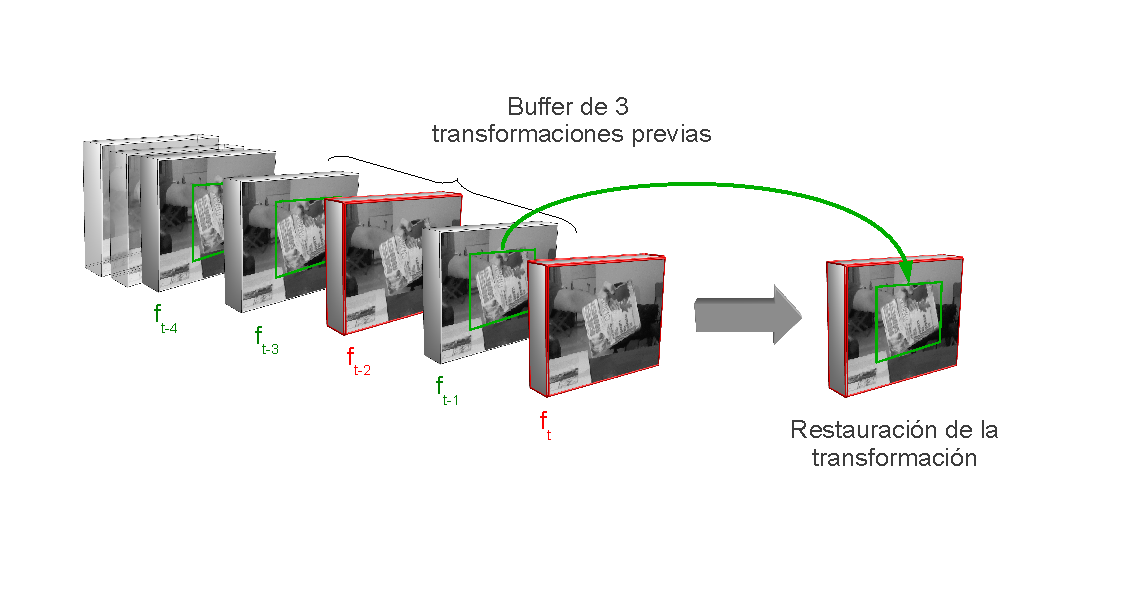
\includegraphics[scale=0.8]{../figs/restauracion_transfromacion}%
\lthtmlpictureZ
\lthtmlcheckvsize\clearpage}

\stepcounter{section}
\stepcounter{subsection}
{\newpage\clearpage
\lthtmlinlinemathA{tex2html_wrap_inline13593}%
$ H$%
\lthtmlinlinemathZ
\lthtmlcheckvsize\clearpage}

{\newpage\clearpage
\lthtmlinlinemathA{tex2html_wrap_inline13597}%
$ (H^{-1})$%
\lthtmlinlinemathZ
\lthtmlcheckvsize\clearpage}

{\newpage\clearpage
\lthtmlpictureA{tex2html_wrap13603}%
\includegraphics[scale=0.75]{../figs/transfperspectiva}%
\lthtmlpictureZ
\lthtmlcheckvsize\clearpage}

\stepcounter{chapter}
\stepcounter{section}
{\newpage\clearpage
\lthtmlinlinemathA{tex2html_wrap_inline13615}%
$ 22cm. \times 17cm.$%
\lthtmlinlinemathZ
\lthtmlcheckvsize\clearpage}

{\newpage\clearpage
\lthtmlinlinemathA{tex2html_wrap_inline13617}%
$ (B_{N})$%
\lthtmlinlinemathZ
\lthtmlcheckvsize\clearpage}

{\newpage\clearpage
\lthtmlinlinemathA{tex2html_wrap_inline13619}%
$ 5$%
\lthtmlinlinemathZ
\lthtmlcheckvsize\clearpage}

{\newpage\clearpage
\lthtmlinlinemathA{tex2html_wrap_inline13621}%
$ d4$%
\lthtmlinlinemathZ
\lthtmlcheckvsize\clearpage}

{\newpage\clearpage
\lthtmlinlinemathA{tex2html_wrap_inline13623}%
$ 1.7$%
\lthtmlinlinemathZ
\lthtmlcheckvsize\clearpage}

{\newpage\clearpage
\lthtmlinlinemathA{tex2html_wrap_inline13625}%
$ d2$%
\lthtmlinlinemathZ
\lthtmlcheckvsize\clearpage}

{\newpage\clearpage
\lthtmlinlinemathA{tex2html_wrap_inline13627}%
$ 0.4$%
\lthtmlinlinemathZ
\lthtmlcheckvsize\clearpage}

{\newpage\clearpage
\lthtmlinlinemathA{tex2html_wrap_inline13629}%
$ d3$%
\lthtmlinlinemathZ
\lthtmlcheckvsize\clearpage}

{\newpage\clearpage
\lthtmlinlinemathA{tex2html_wrap_inline13631}%
$ 0.5$%
\lthtmlinlinemathZ
\lthtmlcheckvsize\clearpage}

{\newpage\clearpage
\lthtmlinlinemathA{tex2html_wrap_inline13633}%
$ d1$%
\lthtmlinlinemathZ
\lthtmlcheckvsize\clearpage}

{\newpage\clearpage
\lthtmlinlinemathA{tex2html_wrap_inline13637}%
$ 0.6$%
\lthtmlinlinemathZ
\lthtmlcheckvsize\clearpage}

{\newpage\clearpage
\lthtmlinlinemathA{tex2html_wrap_inline13639}%
$ (B_{H})$%
\lthtmlinlinemathZ
\lthtmlcheckvsize\clearpage}

{\newpage\clearpage
\lthtmlinlinemathA{tex2html_wrap_inline13641}%
$ (B_{L})$%
\lthtmlinlinemathZ
\lthtmlcheckvsize\clearpage}

{\newpage\clearpage
\lthtmlpictureA{tex2html_wrap13645}%
\includegraphics[scale=0.5]{../figs/entorno/entorno_pruebas}%
\lthtmlpictureZ
\lthtmlcheckvsize\clearpage}

\stepcounter{section}
\stepcounter{subsection}
{\newpage\clearpage
\lthtmlpictureA{tex2html_wrap13662}%

\includegraphics[width=2.5in]{../exp1/train_normal_BN/train_normal}%
\lthtmlpictureZ
\lthtmlcheckvsize\clearpage}

{\newpage\clearpage
\lthtmlpictureA{tex2html_wrap13665}%
\includegraphics[width=2.5in]{../exp1/train_brillante_BH/train_brillante}%
\lthtmlpictureZ
\lthtmlcheckvsize\clearpage}

{\newpage\clearpage
\lthtmlpictureA{tex2html_wrap13668}%
\includegraphics[width=2.5in]{../exp1/train_oscura_BL/train_oscura}%
\lthtmlpictureZ
\lthtmlcheckvsize\clearpage}

{\newpage\clearpage
\lthtmlinlinemathA{tex2html_wrap_inline13685}%
$ 1$%
\lthtmlinlinemathZ
\lthtmlcheckvsize\clearpage}

{\newpage\clearpage
\lthtmlinlinemathA{tex2html_wrap_indisplay13687}%
$\displaystyle \begin{bmatrix} \quad0 & -1 & \quad0\\-1 & \quad5 & -1\\\quad0 & -1 & \quad0 \end{bmatrix}$%
\lthtmlindisplaymathZ
\lthtmlcheckvsize\clearpage}

{\newpage\clearpage
\lthtmlinlinemathA{tex2html_wrap_inline13689}%
$ A=2$%
\lthtmlinlinemathZ
\lthtmlcheckvsize\clearpage}

{\newpage\clearpage
\lthtmlinlinemathA{tex2html_wrap_indisplay13691}%
$\displaystyle \begin{bmatrix} -1 & -1 & -1\\-1 & \quad8 & -1\\-1 & -1 & -1 \end{bmatrix}$%
\lthtmlindisplaymathZ
\lthtmlcheckvsize\clearpage}

{\newpage\clearpage
\lthtmlpictureA{tex2html_wrap13694}%
\includegraphics[width=2.5in]{../exp1/train_normal_BN/train_normal_grises}%
\lthtmlpictureZ
\lthtmlcheckvsize\clearpage}

{\newpage\clearpage
\lthtmlpictureA{tex2html_wrap13695}%
\includegraphics[width=2.5in]{../exp1/train_normal_BN/train_normal_515}%
\lthtmlpictureZ
\lthtmlcheckvsize\clearpage}

{\newpage\clearpage
\lthtmlpictureA{tex2html_wrap13696}%
\includegraphics[width=2.5in]{../exp1/train_normal_BN/keypoints2}%
\lthtmlpictureZ
\lthtmlcheckvsize\clearpage}

{\newpage\clearpage
\lthtmlpictureA{tex2html_wrap13697}%
\includegraphics[width=2.5in]{../exp1/train_normal_BN/keypoints3}%
\lthtmlpictureZ
\lthtmlcheckvsize\clearpage}

{\newpage\clearpage
\lthtmlpictureA{tex2html_wrap13698}%
\includegraphics[width=2.5in]{../exp1/train_normal_BN/keypoints4}%
\lthtmlpictureZ
\lthtmlcheckvsize\clearpage}

{\newpage\clearpage
\lthtmlpictureA{tex2html_wrap13699}%
\includegraphics[width=2.5in]{../exp1/train_normal_BN/keypoints5}%
\lthtmlpictureZ
\lthtmlcheckvsize\clearpage}

{\newpage\clearpage
\lthtmlpictureA{tex2html_wrap13709}%
\includegraphics[width=2.5in]{../exp1/train_brillante_BH/train_brillante_grises}%
\lthtmlpictureZ
\lthtmlcheckvsize\clearpage}

{\newpage\clearpage
\lthtmlpictureA{tex2html_wrap13710}%
\includegraphics[width=2.5in]{../exp1/train_brillante_BH/train_brillante622}%
\lthtmlpictureZ
\lthtmlcheckvsize\clearpage}

{\newpage\clearpage
\lthtmlpictureA{tex2html_wrap13711}%
\includegraphics[width=2.5in]{../exp1/train_brillante_BH/keypoints2}%
\lthtmlpictureZ
\lthtmlcheckvsize\clearpage}

{\newpage\clearpage
\lthtmlpictureA{tex2html_wrap13712}%
\includegraphics[width=2.5in]{../exp1/train_brillante_BH/keypoints3}%
\lthtmlpictureZ
\lthtmlcheckvsize\clearpage}

{\newpage\clearpage
\lthtmlpictureA{tex2html_wrap13713}%
\includegraphics[width=2.5in]{../exp1/train_brillante_BH/keypoints4}%
\lthtmlpictureZ
\lthtmlcheckvsize\clearpage}

{\newpage\clearpage
\lthtmlpictureA{tex2html_wrap13714}%
\includegraphics[width=2.5in]{../exp1/train_brillante_BH/keypoints5}%
\lthtmlpictureZ
\lthtmlcheckvsize\clearpage}

{\newpage\clearpage
\lthtmlpictureA{tex2html_wrap13724}%
\includegraphics[width=2.5in]{../exp1/train_oscura_BL/train_oscura_grises}%
\lthtmlpictureZ
\lthtmlcheckvsize\clearpage}

{\newpage\clearpage
\lthtmlpictureA{tex2html_wrap13725}%
\includegraphics[width=2.5in]{../exp1/train_oscura_BL/train_oscura453}%
\lthtmlpictureZ
\lthtmlcheckvsize\clearpage}

{\newpage\clearpage
\lthtmlpictureA{tex2html_wrap13726}%
\includegraphics[width=2.5in]{../exp1/train_oscura_BL/keypoints2}%
\lthtmlpictureZ
\lthtmlcheckvsize\clearpage}

{\newpage\clearpage
\lthtmlpictureA{tex2html_wrap13727}%
\includegraphics[width=2.5in]{../exp1/train_oscura_BL/keypoints3}%
\lthtmlpictureZ
\lthtmlcheckvsize\clearpage}

{\newpage\clearpage
\lthtmlpictureA{tex2html_wrap13728}%
\includegraphics[width=2.5in]{../exp1/train_oscura_BL/keypoints4}%
\lthtmlpictureZ
\lthtmlcheckvsize\clearpage}

{\newpage\clearpage
\lthtmlpictureA{tex2html_wrap13729}%
\includegraphics[width=2.5in]{../exp1/train_oscura_BL/keypoints5}%
\lthtmlpictureZ
\lthtmlcheckvsize\clearpage}

{\newpage\clearpage
\lthtmlinlinemathA{tex2html_wrap_inline13740}%
$ 700$%
\lthtmlinlinemathZ
\lthtmlcheckvsize\clearpage}

{\newpage\clearpage
\lthtmlpictureA{tex2html_wrap13805}%
\includegraphics[scale=0.75]{../pruebas_modif/graph_ptos_realces}%
\lthtmlpictureZ
\lthtmlcheckvsize\clearpage}

\stepcounter{subsection}
{\newpage\clearpage
\lthtmlinlinemathA{tex2html_wrap_inline13850}%
$ FPS_{prom}$%
\lthtmlinlinemathZ
\lthtmlcheckvsize\clearpage}

{\newpage\clearpage
\lthtmlinlinemathA{tex2html_wrap_inline13854}%
$ 6.93$%
\lthtmlinlinemathZ
\lthtmlcheckvsize\clearpage}

{\newpage\clearpage
\lthtmlinlinemathA{tex2html_wrap_inline13856}%
$ 28.35$%
\lthtmlinlinemathZ
\lthtmlcheckvsize\clearpage}

{\newpage\clearpage
\lthtmlpictureA{tex2html_wrap13866}%
\includegraphics[scale=0.45]{../pruebas_modif/3500_sinproc/graph_tiempos_3500_presentacion1}%
\lthtmlpictureZ
\lthtmlcheckvsize\clearpage}

{\newpage\clearpage
\lthtmlpictureA{tex2html_wrap13871}%
\includegraphics[width=2.5in]{../pruebas_modif/capturas/usables/train_normal}%
\lthtmlpictureZ
\lthtmlcheckvsize\clearpage}

{\newpage\clearpage
\lthtmlpictureA{tex2html_wrap13872}%
\includegraphics[width=2.5in]{../pruebas_modif/capturas/usables/pinguino}%
\lthtmlpictureZ
\lthtmlcheckvsize\clearpage}

{\newpage\clearpage
\lthtmlpictureA{tex2html_wrap13873}%
\includegraphics[width=2.5in]{../pruebas_modif/capturas/usables/captured154}%
\lthtmlpictureZ
\lthtmlcheckvsize\clearpage}

{\newpage\clearpage
\lthtmlpictureA{tex2html_wrap13874}%
\includegraphics[width=2.5in]{../pruebas_modif/capturas/usables/captured135}%
\lthtmlpictureZ
\lthtmlcheckvsize\clearpage}

{\newpage\clearpage
\lthtmlpictureA{tex2html_wrap13875}%
\includegraphics[width=2.5in]{../pruebas_modif/capturas/usables/captured141}%
\lthtmlpictureZ
\lthtmlcheckvsize\clearpage}

{\newpage\clearpage
\lthtmlpictureA{tex2html_wrap13876}%
\includegraphics[width=2.5in]{../pruebas_modif/capturas/usables/captured207}%
\lthtmlpictureZ
\lthtmlcheckvsize\clearpage}

\stepcounter{section}
{\newpage\clearpage
\lthtmlpictureA{tex2html_wrap13883}%
\includegraphics[width=2.5in]{../imgvitina/vitina}%
\lthtmlpictureZ
\lthtmlcheckvsize\clearpage}

{\newpage\clearpage
\lthtmlpictureA{tex2html_wrap13884}%
\includegraphics[width=2.5in]{../imgvitina/preciosvirtuales}%
\lthtmlpictureZ
\lthtmlcheckvsize\clearpage}

{\newpage\clearpage
\lthtmlpictureA{tex2html_wrap13885}%
\includegraphics[width=2.5in]{../imgvitina/captured87,000000}%
\lthtmlpictureZ
\lthtmlcheckvsize\clearpage}

{\newpage\clearpage
\lthtmlpictureA{tex2html_wrap13886}%
\includegraphics[width=2.5in]{../imgvitina/captured94,000000}%
\lthtmlpictureZ
\lthtmlcheckvsize\clearpage}

{\newpage\clearpage
\lthtmlpictureA{tex2html_wrap13887}%
\includegraphics[width=2.5in]{../imgvitina/captured146,000000}%
\lthtmlpictureZ
\lthtmlcheckvsize\clearpage}

{\newpage\clearpage
\lthtmlpictureA{tex2html_wrap13888}%
\includegraphics[width=2.5in]{../imgvitina/captured176,000000}%
\lthtmlpictureZ
\lthtmlcheckvsize\clearpage}

\stepcounter{chapter}
\stepcounter{section}
\stepcounter{section}

\end{document}
